% !TEX program = pdflatex
% IEEE Transactions on Industrial Informatics manuscript
\IfFileExists{ieeecolor.cls}{%
    \documentclass[journal,twoside,web]{ieeecolor}
    \IfFileExists{generic.sty}{\usepackage{generic}}{}
}{%
    % The TII template bundle is not installed in every TeX distribution.
    % IEEEtran preserves the IEEE journal layout until that bundle is present.
    \documentclass[journal,twoside]{IEEEtran}
}

\usepackage{cite}
\usepackage{amsmath,amssymb,amsfonts}
\usepackage{algorithmic}
\usepackage{graphicx}
\usepackage{textcomp}
\usepackage{booktabs}
\usepackage{tabularx}
\usepackage{array}
\usepackage{makecell}
\usepackage{multirow}
\usepackage[caption=false,font=footnotesize]{subfig}
\usepackage{enumitem}
\usepackage{placeins}
\usepackage{stfloats}
\usepackage{microtype}
\usepackage[hidelinks]{hyperref}

\def\BibTeX{{\rm B\kern-.05em{\sc i\kern-.025em b}\kern-.08em
    T\kern-.1667em\lower.7ex\hbox{E}\kern-.125emX}}

\markboth{IEEE Transactions on Industrial Informatics, Vol. XX, No. XX, 2026}
{Author One \MakeLowercase{\textit{et al.}}: CLoMA-UWR: LLM-Centered Closed-Loop Multiagent Framework for Multi-UAV Wildfire Rescue}

\begin{document}

\title{CLoMA-UWR: LLM-Centered Closed-Loop Multiagent Framework for Multi-UAV Wildfire Rescue}

\author{Author One and Author Two%
\thanks{Manuscript received Month XX, 2026; revised Month XX, 2026.}%
\thanks{Author One and Author Two are with the Department, Institution, City,
Postal Code, Country (e-mail: author@example.com).}}

\maketitle

\begin{abstract}
Reliable multi-UAV wildfire rescue requires closed-loop decision making that
converts uncertain aerial observations into executable fleet plans and
preserves mission continuity under runtime perturbations.
Existing UAV approaches commonly optimize perception, navigation, or task
allocation as separate capabilities, leaving a gap between fire-situation
understanding, resource-constrained mission planning, and runtime replanning.
To close this gap, we develop CLoMA-UWR, an LLM-centered closed-loop multiagent
framework for multi-UAV wildfire rescue. CLoMA-UWR transforms aerial
observations into initial mission plans through Vision Analysis and Mission Planning,
audits candidate plans through Validation, uses Memory to inform subsequent
decisions, and invokes Runtime Replanning after runtime perturbations. A
real-UAV-informed AirSim suite evaluates it across four difficulty levels with
resource limitations, scheduling constraints, and runtime perturbations. Across
four downstream foundation-model configurations, CLoMA-UWR outperforms an
Optimization-Based Planner in task completion and execution quality under hard
and expert conditions. Controlled ablations identify the condition-dependent
roles of Validation, Memory, and Runtime Replanning. On simple and normal episodes, a
fine-tuned Qwen3-8B planner retains 98.24\% of the Gemini~3.1~Pro teacher
planner's average score while reducing mean planning time from 37.50 to
14.01~s and mean planning-token usage from 13,353 to 3,593. These results
demonstrate the effectiveness of CLoMA-UWR for adaptive multi-UAV wildfire
rescue.
The implementation is available at \url{https://github.com/tongsuhdyem/Pipeline}.
\end{abstract}

\begin{IEEEkeywords}
Closed-loop decision making, large language model agents, multi-UAV systems,
real-to-simulation evaluation, wildfire rescue.
\end{IEEEkeywords}

% !TEX root = ../main.tex
\section{Introduction}
\label{sec:introduction}

\IEEEPARstart{W}{ildfires} threaten ecosystems, infrastructure, and human safety
\cite{bowman2020wildfire}. UAVs can rapidly observe hazardous and inaccessible
areas through flexible aerial sensing \cite{allan2022remote}, but operational
response requires observations to be converted into task zones, assigned across
a resource-limited fleet, and revised as the fire or UAV state changes.
Multi-UAV wildfire rescue is therefore a closed-loop decision problem rather
than an isolated perception or path-planning task.

An initial mission must be feasible for the current fleet: task priorities must
be matched to vehicle locations, endurance, payload, communication, and safety
limits \cite{floreano2015science}. Feasibility is also temporary because fire
evolution, resource consumption, communication changes, and UAV faults can
invalidate existing assignments. Initial resource-constrained mission planning
and runtime replanning must consequently be treated as coupled parts of the
same decision problem.

Existing work has advanced the individual capabilities needed for this process
\cite{erdelj2017help}. Thermal--RGB fusion, aerial semantic segmentation, and
learning-based 3D reconstruction improve fire detection and scene modeling
\cite{yuan2021uavfire,zhang2022uavtransformer,
yang2022uav3dreconstruction}, while autonomous exploration and mapping and
next-best-view planning update environmental knowledge and reduce observation
uncertainty \cite{popovic2021uavdisaster,bircher2016nbv}. On the action side,
deep reinforcement learning and coverage path planning support navigation and
large-area search \cite{xiao2021uavrl,yu2022coverageuav}, whereas multi-agent
reinforcement learning and human--robot collaboration support task allocation
and search-and-rescue operations
\cite{yang2023multiagentuav,waharte2021uavsar}. However, these capabilities are
commonly optimized and evaluated separately, often from a fixed initial state.
They therefore do not establish how visual and spatial evidence can be converted
into fire points and task zones for resource-constrained mission planning, or
how an initially feasible allocation should be revised when the fire, fleet, or
resource state changes.

Large language models (LLMs) provide a flexible interface between high-level
intent, structured observations, and robot behavior. SayCan grounds instructions
in executable skills \cite{ahn2022saycan}, Code as Policies generates
programmatic control policies \cite{liang2023codeaspolicies}, and related design
guidance exposes tools and environmental constraints to ChatGPT-generated robot
workflows \cite{vemprala2023chatgptrobotics}. Embodied and multimodal models
further connect reasoning to physical state: RT-1 learns vision-language-action
policies \cite{brohan2023rt1}, PaLM-E incorporates visual inputs and robot states
\cite{driess2023palme}, and Socratic Models compose specialized vision and
language models \cite{zeng2023socratic}. These approaches support task
decomposition and action sequencing, but they also show that generated actions
require grounding and external feasibility checks. Embodied and multimodal
models are generally evaluated on individual robots and predefined manipulation
or navigation tasks. Moving to a fleet-level decision layer introduces coupling
among vehicle states, task priorities, routes, and shared resources; linguistic
coherence therefore does not ensure that assignments jointly respect
endurance, payload, communication, priority, and safety constraints.

LLM-based agents have also used environmental feedback and accumulated
experience for sequential decision making. Inner Monologue revises embodied
plans from language-based feedback \cite{huang2023innermonologue}, LM-Nav uses
semantic waypoints for open-world navigation \cite{shah2023lmnav}, and Voyager
combines an LLM agent with an automatic curriculum and a growing skill library
\cite{wang2023voyager}. These systems primarily target single-agent embodied
environments rather than dynamic, interdependent tasks across a
resource-constrained fleet. They establish that feedback and accumulated
experience can improve sequential behavior, but do not establish how these
capabilities should be combined with fleet-wide resource constraints or how
their importance changes as operational pressure increases. Existing research
therefore provides the main ingredients for perception, planning, coordination,
and feedback, but not a common high-level decision loop that connects
fire-situation understanding, resource-constrained mission planning,
Validation, Memory, and Runtime Replanning. Strong perception does not by
itself establish that detected fire conditions can be converted into a feasible
fleet mission, while a feasible initial mission plan does not establish that the
mission can remain effective under subsequent perturbations. The central
question is whether LLMs can serve as the high-level closed-loop decision core
of a multi-UAV wildfire rescue system, and how Validation, Memory, and Runtime
Replanning sustain that role as operational pressure increases.

We address this question with an LLM-centered closed-loop decision framework
that transforms aerial observations through Vision Analysis and Mission
Planning into an initial fleet mission. Semantic Validation and Deterministic
Rule Validation reject plans that are tactically implausible or structurally
invalid, converting validation failures into targeted feedback for Mission
Planning. Episodic Memory retrieves concrete prior cases, whereas Lesson Memory
provides distilled guidance about recurring planning and resource-management
patterns. Runtime Replanning repairs the affected part of the active mission
after changes in the fire, fleet, resources, or schedule. Together, these
mechanisms turn one-shot LLM planning into a decision process that connects
fire-situation understanding, resource-constrained mission planning,
Validation, execution feedback, and Runtime Replanning within one continuous
loop.

We evaluate the framework in a real-UAV-informed AirSim suite through
end-to-end comparisons, controlled ablations, and compact-planner fine-tuning.

The main contributions of this work are summarized as follows:
\begin{enumerate}[leftmargin=1.6em,itemsep=2pt,topsep=3pt]
    \item We formulate resource-constrained multi-UAV wildfire rescue as a
    high-level closed-loop decision problem and develop an LLM-centered
    closed-loop decision framework that connects fire-situation understanding
    and resource-constrained mission planning with Validation, Memory, and
    Runtime Replanning.
    \item We construct a real-UAV-informed AirSim evaluation suite that exposes
    the decision loop to controlled increases in operational pressure through
    resource limitations, scheduling constraints, and runtime perturbations
    across four difficulty levels, and measures both task completion and
    execution quality with six mission-level metrics.
    \item We evaluate end-to-end behavior against an Optimization-Based Planner
    and across multiple foundation-model configurations, characterize through
    controlled ablations how Validation, Memory, and Runtime Replanning
    contribute as operational pressure increases, and assess whether validated
    demonstrations can specialize a compact planner with lower planning
    overhead.
\end{enumerate}

\endinput

\section{CLoMA-UWR Framework}
\label{sec:system-design}

This section formulates multi-UAV wildfire rescue as a sequence from
fire-situation understanding to resource-constrained mission planning and
runtime replanning, and presents CLoMA-UWR as the framework that implements this
sequence. The task model represents aerial observations,
fire points, task zones, UAV operational states, mission constraints, runtime
perturbations, and the corresponding initial and revised mission plans. It
exposes three decision risks: a generated plan may violate tactical or structural
constraints, one-shot reasoning may fail to use relevant prior experience, and
an initially feasible plan may become obsolete during execution. As shown in
Figure~\ref{fig:method-overview}, Vision Analysis and Mission Planning construct
candidate plans, Validation checks them before execution, Memory supplies prior
experience, and Runtime Replanning revises the active mission after operational
state changes. The following subsections detail the task model and system
components.

\subsection{Task Modeling}

For each mission, the rescue world is represented by the structured state $S$:
\[
S=\{O,F,R,U,C,E\}.
\]
Here, $O$ denotes aerial observations; $F$ denotes fire points; $R$ denotes
task zones; $U$ denotes UAV operational states; $C$ denotes mission constraints;
and $E$ denotes runtime perturbations. This representation
separates the underlying rescue world from the information available to the
decision system. At mission start, the system receives the initial input
$X_0=\{O,U,C\}$, whereas $F$ and $R$ must be inferred from the observation. 
When a runtime perturbation occurs, it receives the updated operational 
state $U_t$ and the observed perturbation $E_t$. The required outputs are an 
initial mission plan $P$ and, when necessary, a revised plan $P'$.

The resulting task model comprises the following decision chain:
\[
\begin{gathered}
O \rightarrow F \rightarrow R,\qquad (R,U,C) \rightarrow P, \\
(P,U_t,E_t) \rightarrow P'.
\end{gathered}
\]
The first two relations transform raw aerial observations into an actionable
regional representation of the fire situation. The third relation generates an
executable fleet plan under operational constraints. The final relation adapts
that plan to changes encountered during execution. This formulation captures
the continuous rescue workflow while retaining the stage-specific information
needed to design and evaluate a closed-loop system.

\subsection{Proposed Framework}

\begin{figure*}[!t]
    \centering
    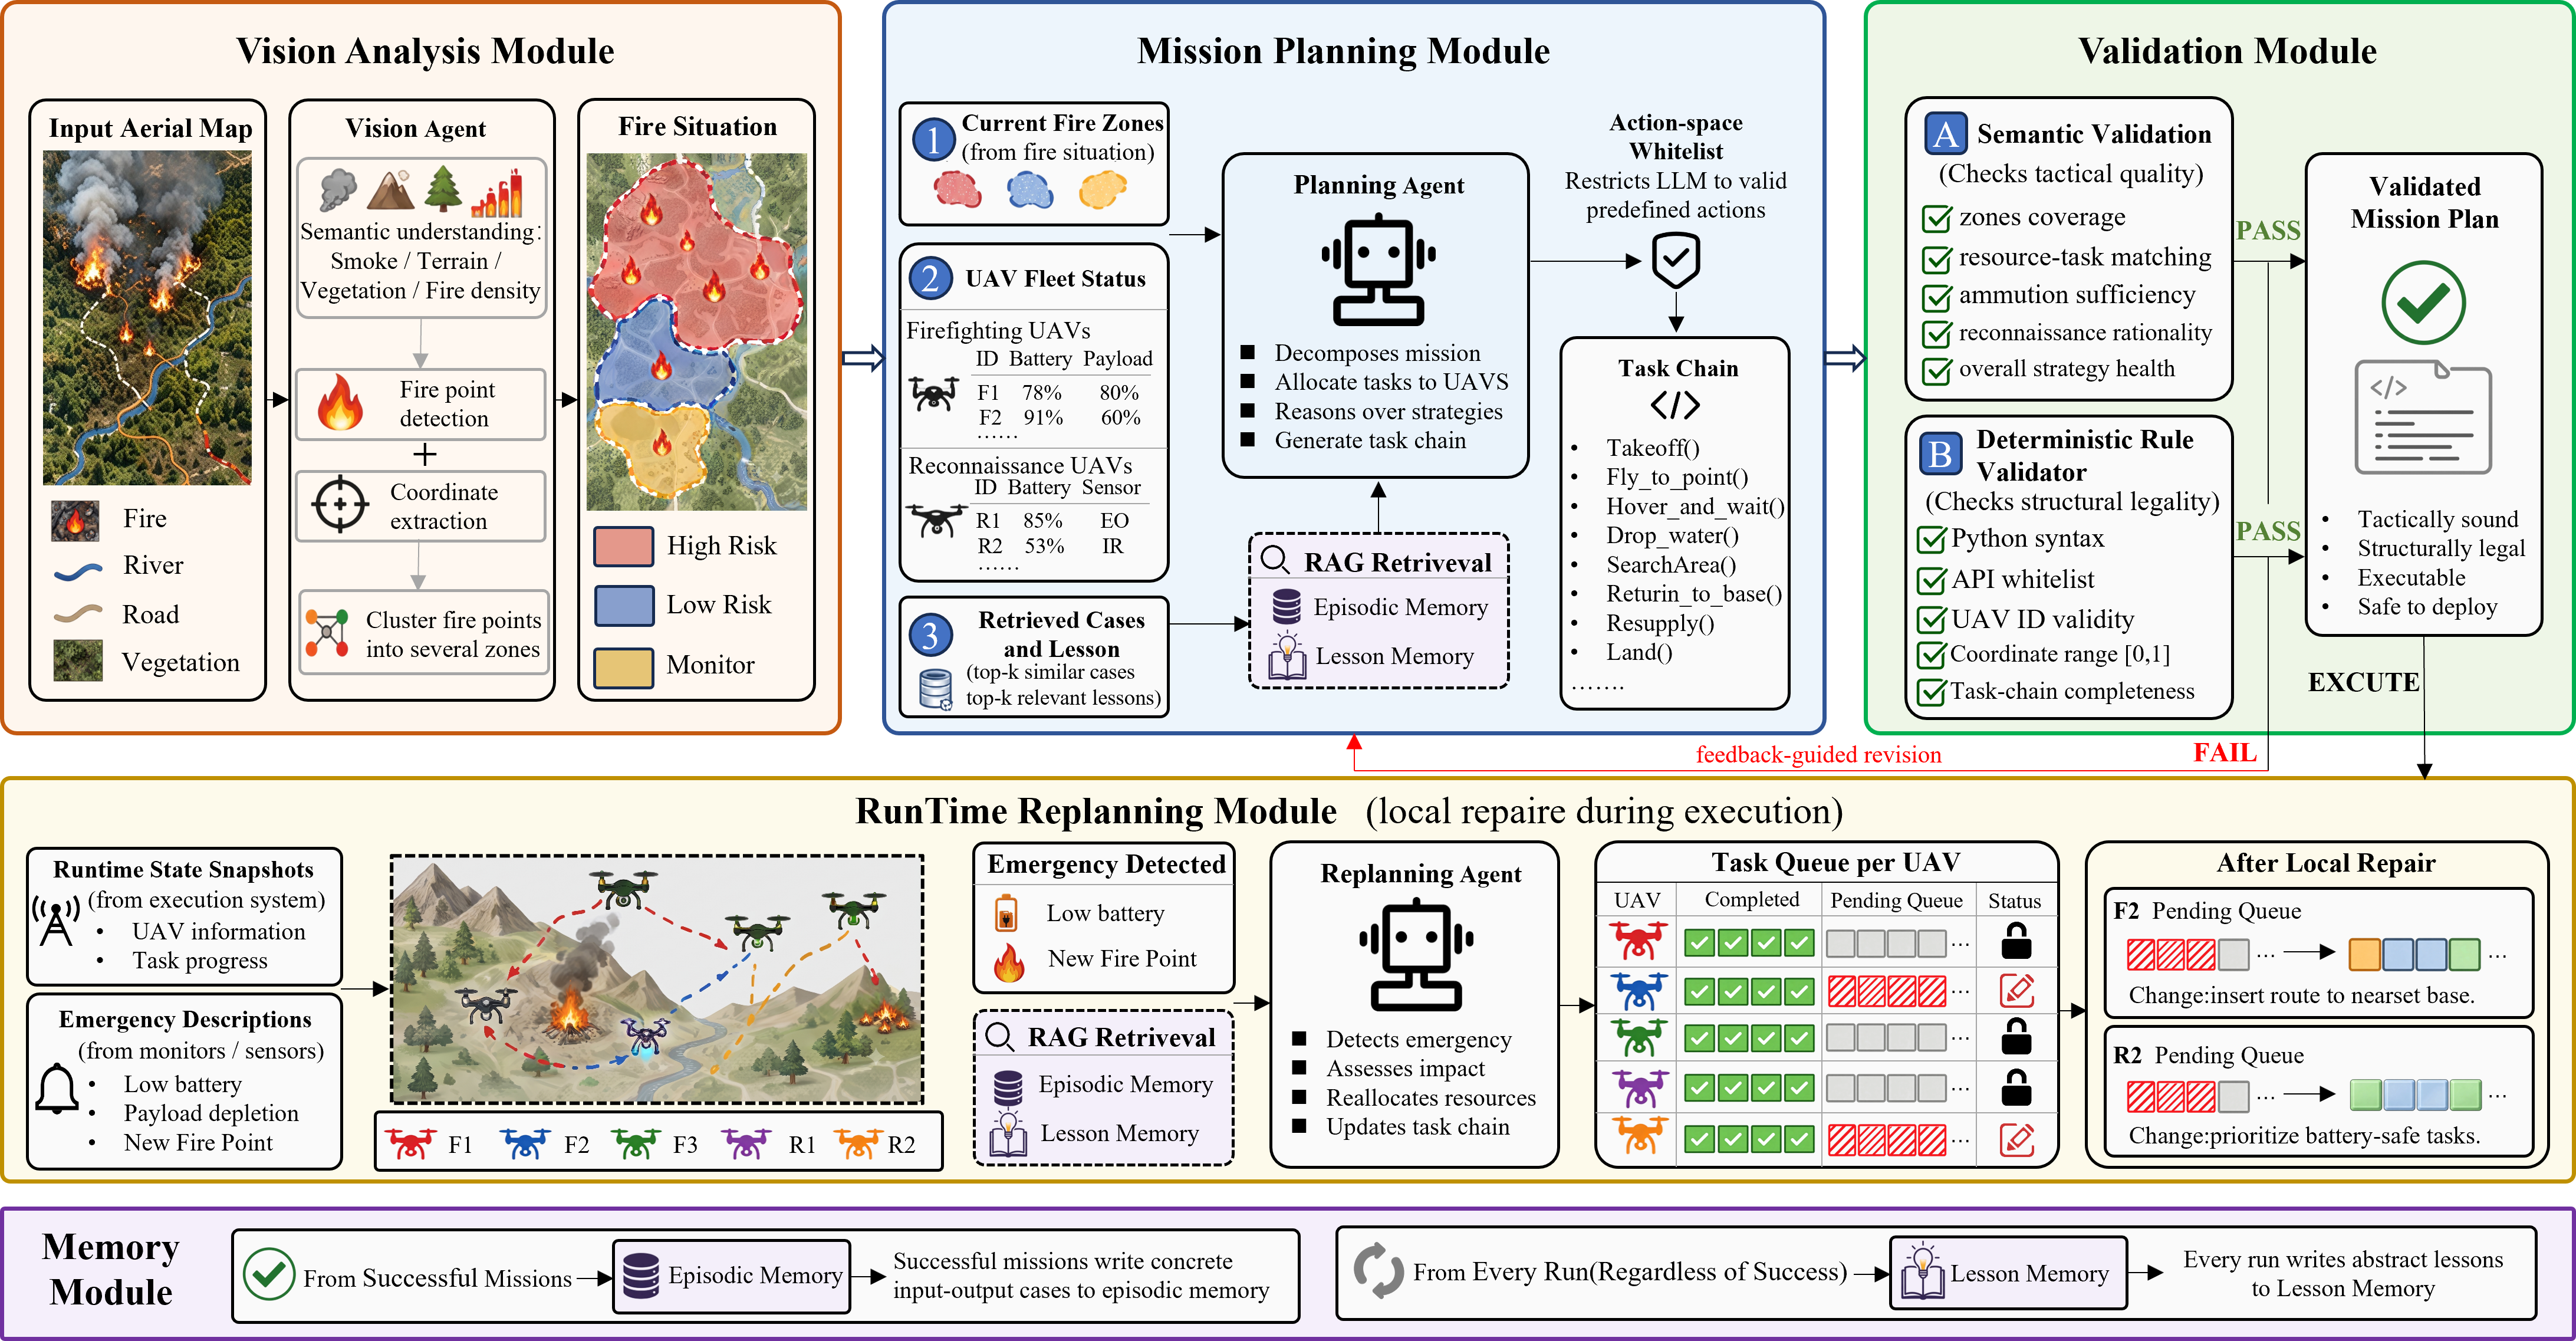
\includegraphics[width=1\textwidth]{figures/system-overview.png}
    \makeatletter
    \long\def\@makecaption#1#2{%
        \@IEEEfigurecaptionsepspace
        \hbox to\hsize{\normalfont\footnotesize\hfil
            \hbox{\normalfont\footnotesize #1.\nobreakspace\nobreakspace #2}\hfil}}
    \makeatother
    \caption{Overview of CLoMA-UWR.}
    \label{fig:method-overview}
\end{figure*}

Figure~\ref{fig:method-overview} summarizes the flow of mission state, candidate
plans, corrective feedback, and prior experience among the CLoMA-UWR components,
whose individual roles are described below.

\paragraph{Vision Analysis} Vision Analysis anchors the decision loop by
reducing the ambiguity between raw aerial observations and the planning state.
It converts raw aerial imagery into a structured description of the fire
situation.
This module uses a multimodal LLM to perform two tasks in a single inference pass.
First, it detects all visible fire points in the image and outputs their normalized coordinates.
Second, it clusters these points by spatial density, partitioning the continuous fire field
into several discrete task zones.

This module uses a multimodal LLM rather than a vision-only model because zone division
depends on more than fire point locations.
The division also depends on visual context, such as smoke, vegetation,
and terrain boundaries.
These cues require joint reasoning over appearance and spatial semantics.
The resulting fire points and task zones provide the shared initial-state
representation used by Mission Planning.

\paragraph{Mission Planning} Mission Planning addresses the fleet-level
coupling among task priorities, vehicle states, and resource constraints. It is
the core decision module and converts the structured fire situation produced by
Vision Analysis into a candidate multi-UAV collaborative plan. A planning LLM
generates a complete task chain for each UAV in the fleet, covering task
allocation, temporal sequencing, and endurance management. To keep outputs
controllable, the LLM is restricted to a predefined set of allowable actions.

Mission Planning combines the fire situation, retrieved experience,
and operational constraints.
It receives the structured fire situation from Vision Analysis,
retrieves relevant prior experience from Memory,
and produces a coordinated plan in which each UAV's task chain respects
the fleet's capabilities and the mission's operational constraints.
Formally, the planning process is expressed as
\begin{equation}
P=\mathcal{G}\bigl(R,U,C,M(q)\bigr),
\qquad q=q(R,U,C),
\label{eq:memory-augmented-planning}
\end{equation}
where $\mathcal{G}$ denotes the planning LLM, $q(R,U,C)$ denotes the query
construction from the current task zones, fleet states, and constraints, and $M(q)$ 
denotes the prior experience retrieved from Memory for that query.
The resulting $P$ is a candidate plan rather than an automatically trusted
output; it is passed to Validation before mission execution.

\paragraph{Validation} Validation addresses the risk that a linguistically
coherent candidate plan may still be tactically implausible or structurally
invalid. It evaluates tactical rationality and structural legality, including
zone coverage completeness, resource-task matching, payload adequacy, UAV
existence, coordinate validity, and task-chain completeness. When Validation
rejects a plan, its feedback is routed back to Mission Planning as targeted
guidance for revision. Only an accepted plan proceeds to execution, preserving
the separation between plan generation and plan acceptance.


\paragraph{Runtime Replanning} Runtime Replanning addresses the risk that an
accepted plan becomes invalid after the operational state changes. This module
handles runtime perturbations during mission execution.
It takes a runtime state snapshot as input, including current positions, battery levels,
payloads, and task progress for each UAV.
Its output is not a new global plan, but a local revision of the current plan.
Unlike the main pipeline, Runtime Replanning reasons about a dynamic execution state and
changes only the affected part of the plan.

When a runtime perturbation occurs, the module retrieves similar prior cases
from Memory as repair references.
These cases describe how comparable failures were resolved in past missions,
providing the replanning LLM with tactical precedents for the current situation.
The resulting local revision closes the execution-feedback loop without
restarting the complete pre-execution pipeline.

\paragraph{Memory} Memory addresses the risk that relevant prior experience is
unavailable when coupled resource, scheduling, or event conditions make the
current decision less routine. It allows the system to reuse past experience.
Each memory entry records a task situation, the generated or revised plan,
validation feedback, runtime perturbations, the execution outcome, and reusable
guidance extracted from the completed mission. Memory is represented as
\begin{equation}
M=\{(z_i,P_i,o_i)\}_{i=1}^{N},
\label{eq:memory-store}
\end{equation}
where $m_i=(z_i,P_i,o_i)$ denotes a memory entry, and $z_i$, $P_i$, and
$o_i$ denote the task situation, the associated plan, and the execution outcome
of completed mission $i$, respectively. Validation feedback, runtime perturbations, 
and reusable guidance are retained as associated information. The system retrieves 
the $K$ most semantically similar entries to the current query according to
\begin{equation}
\begin{aligned}
\mathcal{R}_K(q,M)
&=\underset{m_i\in M}{\operatorname{TopK}}\;
  \operatorname{sim}(q,m_i),\\
\operatorname{sim}(q,m_i)
&=\frac{\phi(q)^\top\phi(m_i)}
{\lVert\phi(q)\rVert_2\lVert\phi(m_i)\rVert_2}.
\end{aligned}
\label{eq:semantic-memory-retrieval}
\end{equation}
where $\mathcal{R}_K(q,M)$ is the set of the $K$ entries retrieved from $M$ for
query $q$, $\phi(\cdot)$ maps a query or memory entry to its semantic embedding. 
The retrieved set provides Mission Planning or Runtime Replanning with concrete 
tacticalprecedents and reusable guidance about recurring planning, resource-management,
and repair patterns.

\endinput

\section{Evaluation Suite Design}
\label{sec:evaluation-suite}

This section presents a controlled, real-UAV-informed evaluation suite in
AirSim for testing whether CLoMA-UWR remains effective as operational pressure
increases. It instantiates the task model in
Section~\ref{sec:system-design} through real-to-sim calibration, difficulty
stratification, and mission-level metrics, which ground the simulated setting,
vary operational pressure, and separate task completion, execution quality, and
mission continuity. As summarized in Table~\ref{tab:benchmark_comparison},
existing settings cover only parts of the transition from aerial observation to
task-zone construction, resource-constrained mission planning, and runtime
replanning; the comparison concerns evaluation coverage rather than algorithmic
performance. The following subsections detail the three design elements.

% Required packages:
% \usepackage{booktabs}
% \usepackage{makecell}
% \usepackage{graphicx}

% Monochrome symbols are clearer and more appropriate for print publication.
\newcommand{\cmark}{\ensuremath{\bullet}}
\newcommand{\pmark}{\ensuremath{\circ}}
\newcommand{\xmark}{\textemdash}

\begin{table}[!t]
\centering
\caption{Coverage of evaluation capabilities in existing datasets, benchmarks,
and the evaluation suite used in this work.
\cmark indicates explicit coverage, \pmark indicates partial coverage, and \xmark indicates no explicit coverage.}
\label{tab:benchmark_comparison}
\footnotesize
\setlength{\tabcolsep}{1.5pt}
\renewcommand{\arraystretch}{1.08}
\begin{tabular}{
    @{}
    >{\raggedright\arraybackslash}p{0.32\columnwidth}
    *{4}{>{\centering\arraybackslash}p{0.14\columnwidth}}
    @{}}
\toprule
\textbf{Benchmark / dataset}
& \textbf{\makecell{Fire\\perc.}}
& \textbf{\makecell{Disaster\\sem.}}
& \textbf{\makecell{UAV\\constr.}}
& \textbf{\makecell{Runtime\\repl.}} \\
\midrule

DOTA~\cite{xia2018dota}
& \cmark & \xmark & \xmark & \xmark \\

VisDrone~\cite{zhu2022visdrone}
& \cmark & \xmark & \xmark & \xmark \\

UAVs-FFDB~\cite{mowla2024uavsffdb}
& \cmark & \cmark & \xmark & \xmark \\

FLAME~\cite{shamsoshoara2021flame}
& \cmark & \cmark & \xmark & \xmark \\

MS-FSDB~\cite{han2024msfsdb}
& \pmark & \cmark & \xmark & \xmark \\

WildFireVQA~\cite{habibpour2026wildfirevqa}
& \cmark & \cmark & \pmark & \xmark \\

RMASBench~\cite{kleiner2013rmasbench}
& \xmark & \cmark & \pmark & \pmark \\

CrisisBench~\cite{alam2021crisisbench}
& \xmark & \cmark & \xmark & \xmark \\

\midrule
\textbf{Our Evaluation Suite}
& \cmark & \cmark & \cmark & \cmark \\

\bottomrule
\end{tabular}
\end{table}


\begin{figure}[!t]
    \centering
    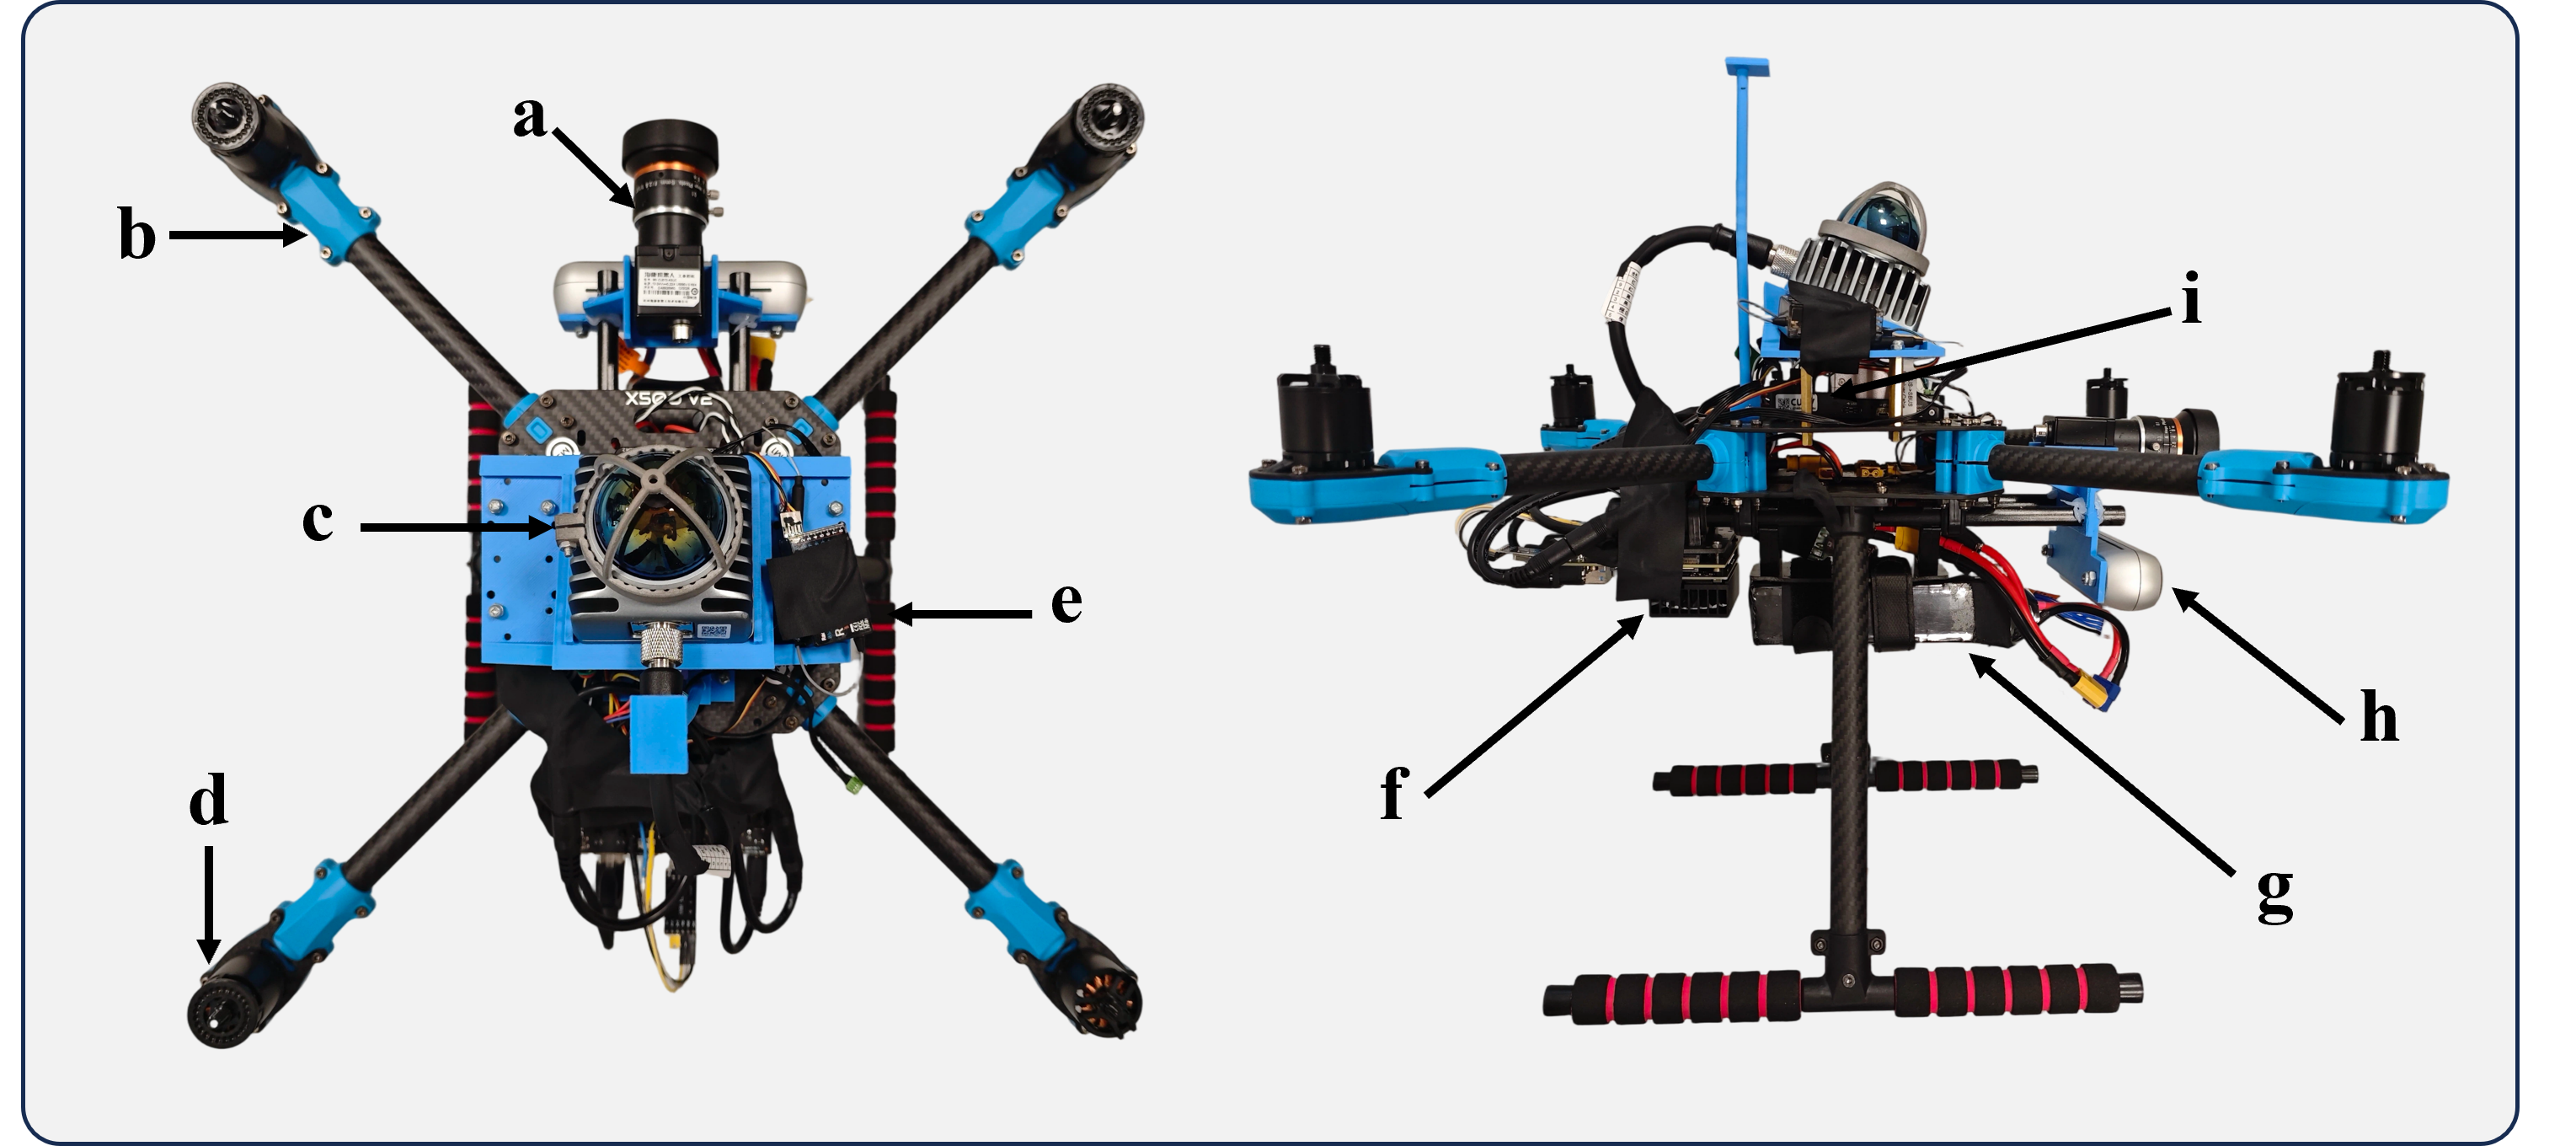
\includegraphics[width=\columnwidth]{figures/real-uav-platform.png}
    \caption{UAV platform and its main components: (a) LiDAR,
    (b) frame, (c) monocular camera, (d) motor, (e) receiver, 
    (f) onboard computer, (g) power supply, 
    (h) stereo camera, and (i) flight controller.}
    \label{fig:UAV-platform}
\end{figure}

\subsection{Real-to-Sim Calibration}
\label{subsec:real-to-sim-calibration}
The first design property is realized through a co-design between the real UAV
platform and the AirSim simulation environment. As stated above, real UAV
parameters constrain every evaluation episode. Accordingly, the real platform defines the
engineering boundary of the rescue mission, while AirSim configures controllable
and repeatable evaluation episodes within that boundary. Rather than treating the two as
separate experimental settings, we use the real platform to define the feasible
set from which AirSim configures each simulated UAV and its environment.
For each UAV, the configured mission must satisfy
\begin{equation}
\begin{aligned}
\mathcal{E}_{\mathrm{UAV}}=\{&(h,v,m,e_{\mathrm{avail}},r)\mid\\
    &h\in \mathcal{H}_{\mathrm{safe}},\quad
      v\in \mathcal{V}_{\mathrm{safe}},\\
    &m\leq m_{\max},\quad
      e_{\mathrm{req}}+e_{\mathrm{res}}\leq e_{\mathrm{avail}},\\
    &r\leq r_{\mathrm{link}}\}.
\end{aligned}
\label{eq:uav-envelope}
\end{equation}
where $\mathcal{E}_{\mathrm{UAV}}$ is the feasible UAV configuration set;
$h$, $v$, $m$, $e_{\mathrm{avail}}$, and $r$ denote flight altitude, velocity,
payload mass, available energy, and communication-link distance,
respectively. $\mathcal{H}_{\mathrm{safe}}$ and
$\mathcal{V}_{\mathrm{safe}}$ are the safe altitude and velocity sets specified
by the operating policy; $m_{\max}$ is the maximum payload mass;
$e_{\mathrm{req}}$ and $e_{\mathrm{res}}$ are the energy required for the
mission and the reserve energy for a safe return; and $r_{\mathrm{link}}$ is the
maximum communication-link distance. These bounds combine hardware
specifications, flight-safety policy, and deployment configuration. Any
configuration that violates
Eq.~\ref{eq:uav-envelope} is excluded before episode generation. The real UAV
platform is shown in Figure~\ref{fig:UAV-platform}, and its hardware
specifications are listed in Table~\ref{tab:real_uav_hardware}.

\input{tables/real-uav-hardware-specifications}

The virtual observation process is further fixed by the real camera geometry.
Under a nadir-view, locally planar-ground approximation, for altitude $h$,
horizontal field of view $\theta_{\mathrm{FOV}}$, and horizontal
resolution $N_x$, the image footprint and ground sampling distance are
\begin{equation}
W(h)=2h\tan\left(\frac{\theta_{\mathrm{FOV}}}{2}\right),\qquad
\mathrm{GSD}(h)=\frac{W(h)}{N_x}.
\label{eq:observation-geometry}
\end{equation}
Thus, the AirSim camera pose and the scale, density, and placement of fire
points are jointly constrained by what the real camera could observe, rather
than selected independently. Energy and payload limits likewise constrain route
length, task duration, and suppressible workload. Table~\ref{tab:real_to_sim_calibration}
records these calibration rules and the resulting simulation settings.

\input{tables/airsim-real-to-sim-calibration}

These calibrated bounds provide the common operational basis on which the
difficulty levels are constructed.

\subsection{Difficulty Stratification}
Each of the four difficulty levels in Table~\ref{tab:scenario-controls}
contains 20 fixed evaluation episodes, yielding 80 episodes in total. The simple
and normal levels test fire-situation understanding and resource-constrained
mission planning without runtime perturbations, whereas the hard and expert
levels introduce progressively stronger resource constraints and scheduling
interactions together with runtime perturbations. All fleet, sensing, energy,
payload, and communication settings
remain within the real-to-sim calibrated bounds in
Section~\ref{subsec:real-to-sim-calibration}.

\input{tables/scenario-difficulty-controls}

The fire-point configurations of all episodes are pre-specified rather than
randomly generated. These configurations control the scene structure
and the spatial arrangement and number of fire points per task zone across
difficulty levels.
Figure~\ref{fig:difficulty-scene-examples} provides representative scenes from
the four difficulty levels, and Figure~\ref{fig:fire-point-count-distribution} summarizes
the distribution of fire-point counts per task zone within each difficulty level. Together,
they illustrate the scene layouts and task-zone-level fire-point distributions
used to instantiate the four difficulty levels.

\begin{figure*}[!t]
    \centering
    \includegraphics[width=1\textwidth]{figures/difficulty-level-fire-scenes.png}
    \caption{Representative fire scenes from the four difficulty levels.
    In each example, \textit{Origin image} denotes the original aerial image,
    and \textit{Perception result} denotes the output generated by the Vision
    Analysis module, which uses Gemini~3.1 Pro as its foundation model.}
    \label{fig:difficulty-scene-examples}
\end{figure*}

\begin{figure}[!t]
    \centering
    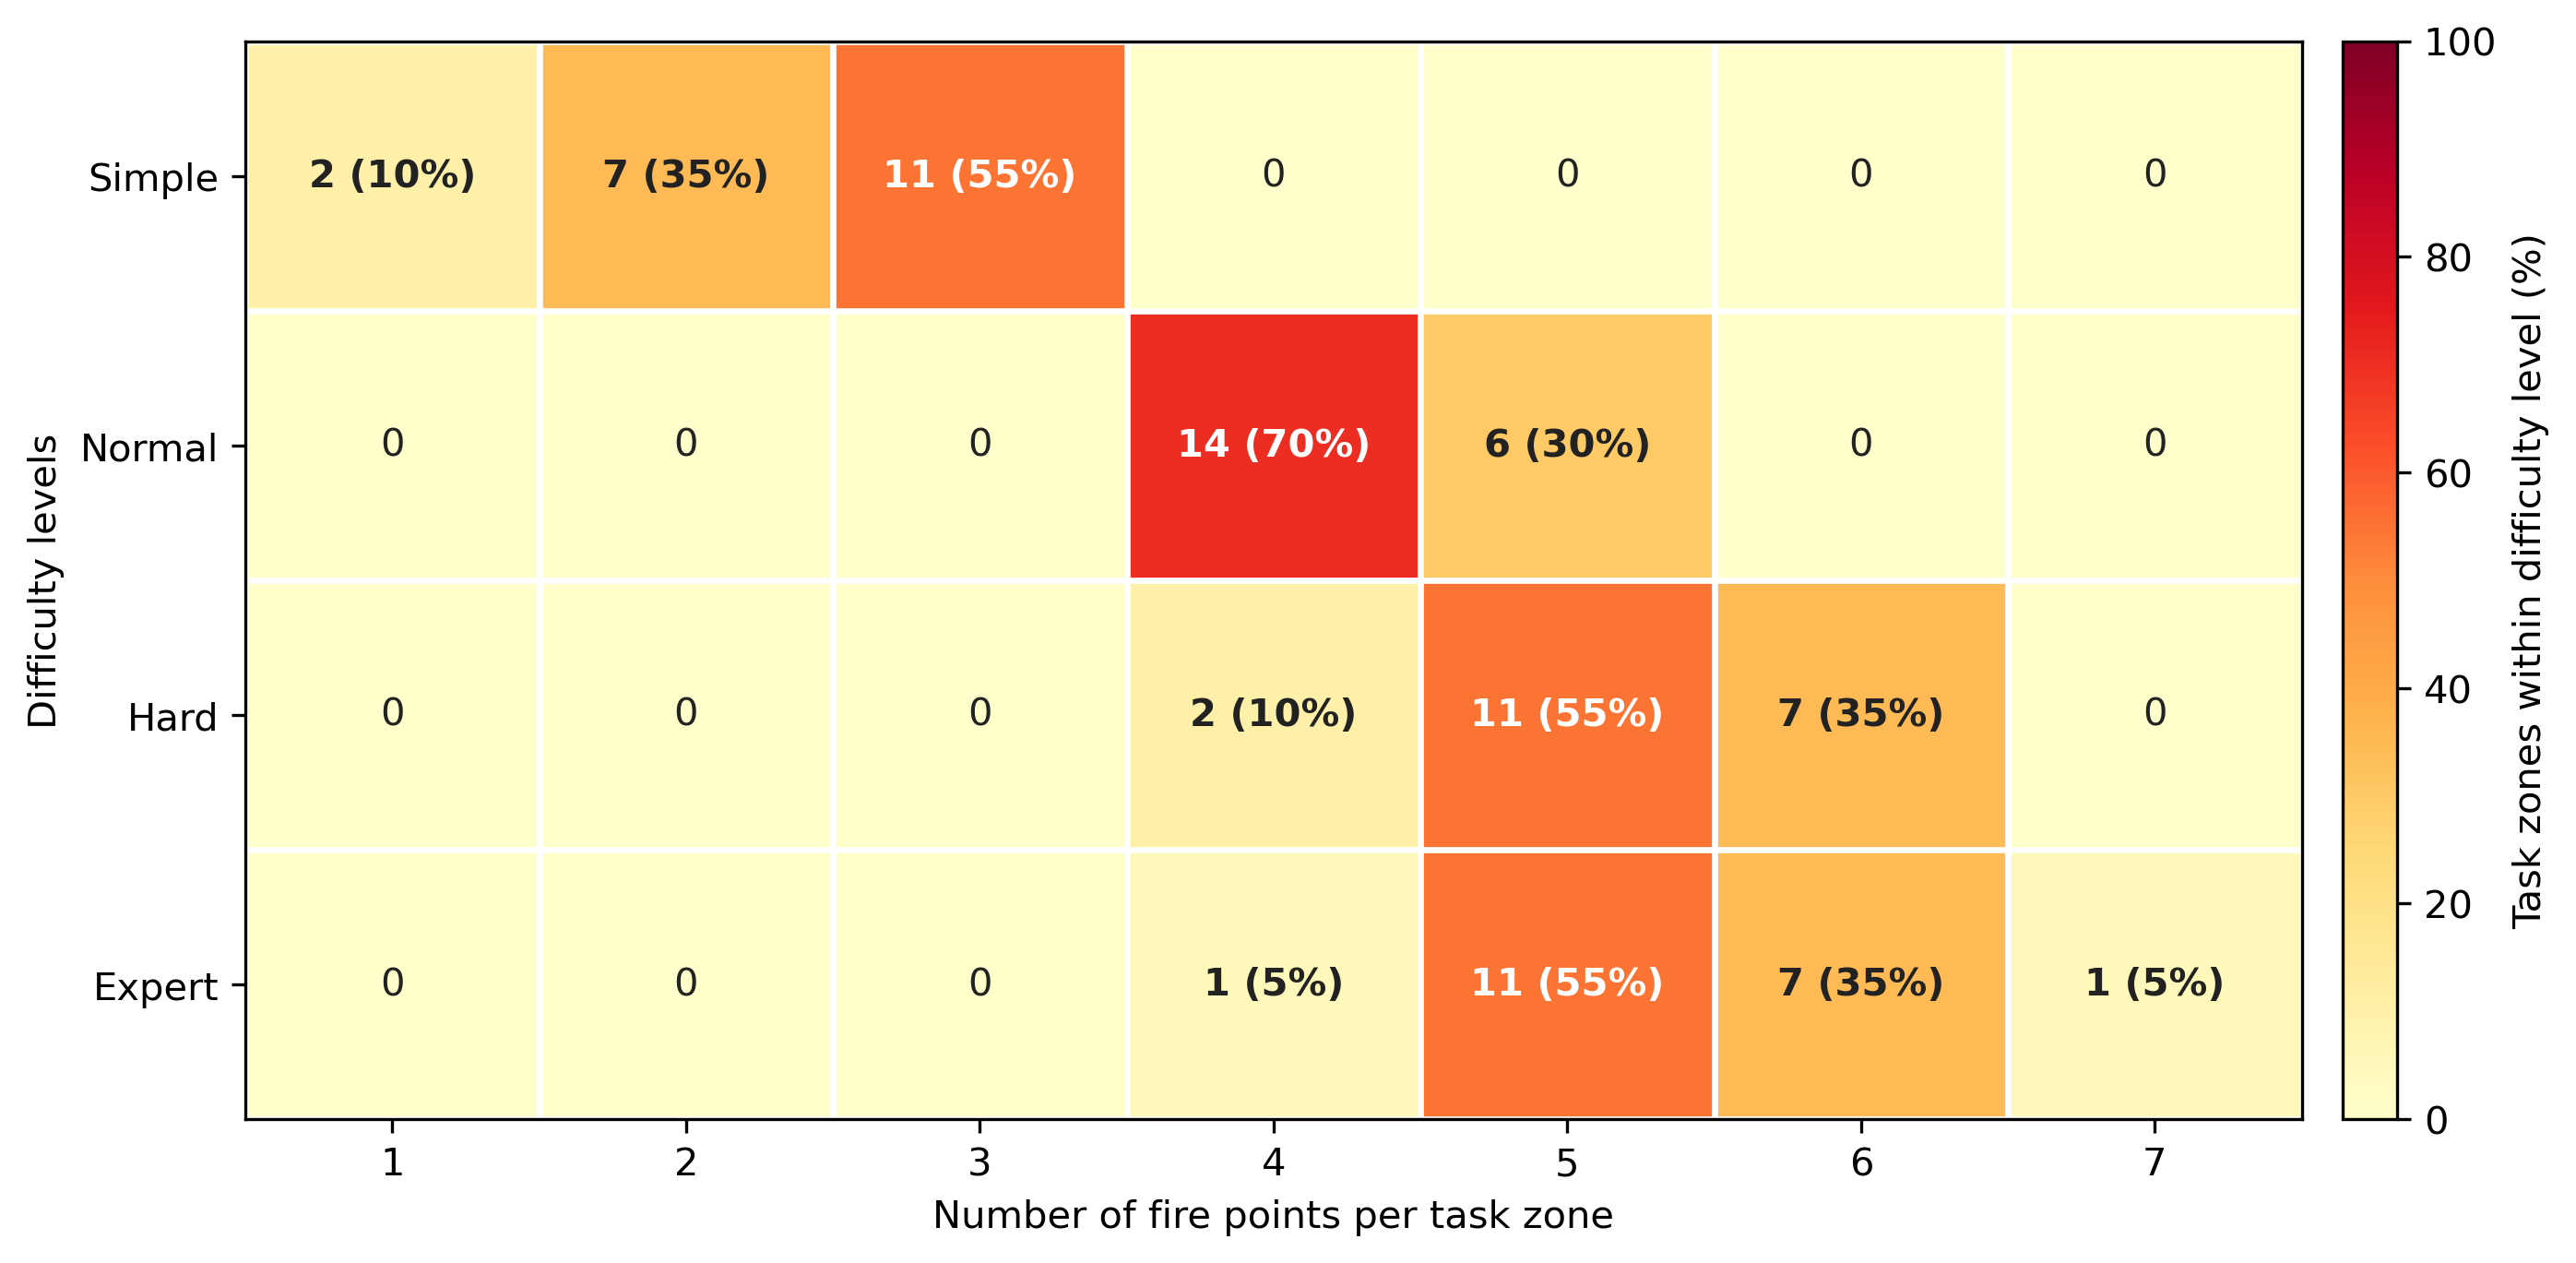
\includegraphics[width=\columnwidth]{figures/task-zone-fire-point-distribution.png}
    \caption{Distribution of fire-point counts per task zone across difficulty
    levels.}
    \label{fig:fire-point-count-distribution}
\end{figure}

Runtime perturbations modify the operational state or mission constraints after
execution begins. Figure~\ref{fig:runtime-perturbation-distribution} summarizes
the five event families and the fixed draws used in hard and expert episodes;
events are sampled once during suite construction and placed at predefined
episode points, with hard episodes using a few temporally separated
perturbations and expert episodes using more frequent, potentially overlapping
perturbations.

\begin{figure*}[!t]
    \centering
    \subfloat[Runtime perturbation library.]{%
        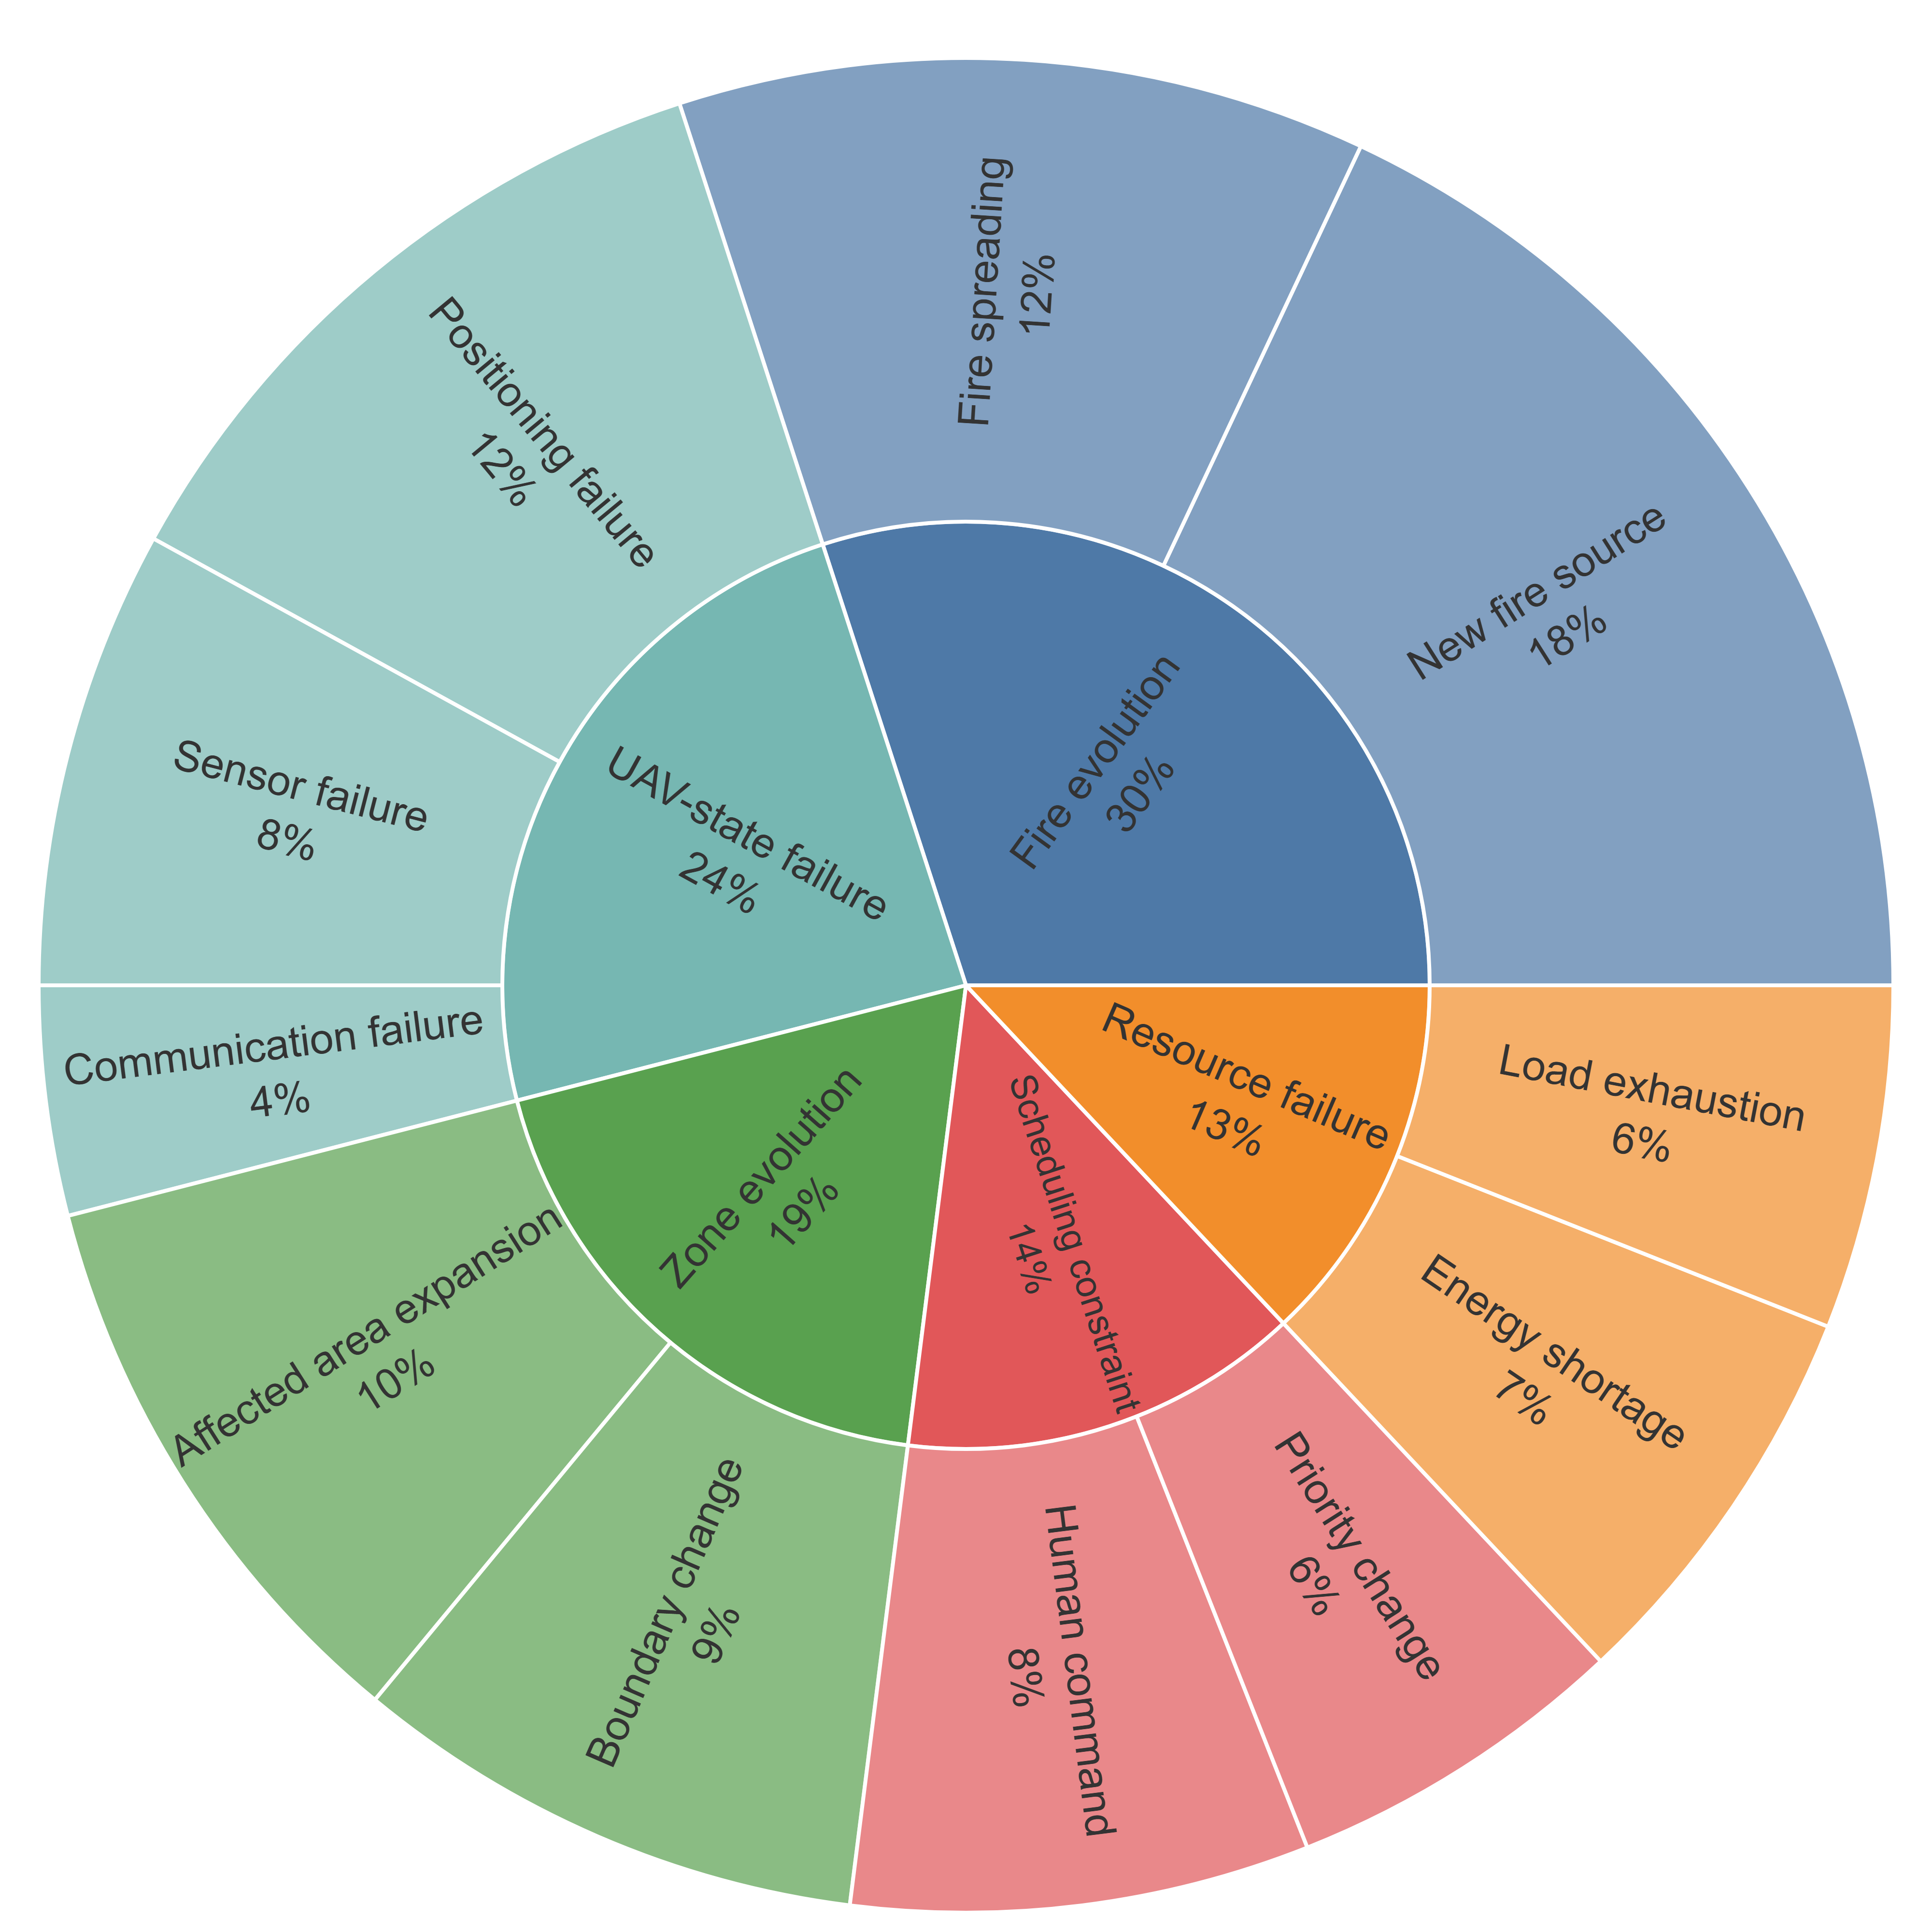
\includegraphics[width=0.35\textwidth]{figures/runtime-perturbation-library.png}}\hspace{0.04\textwidth}
    \subfloat[Distribution of perturbations in hard and expert levels.]{%
        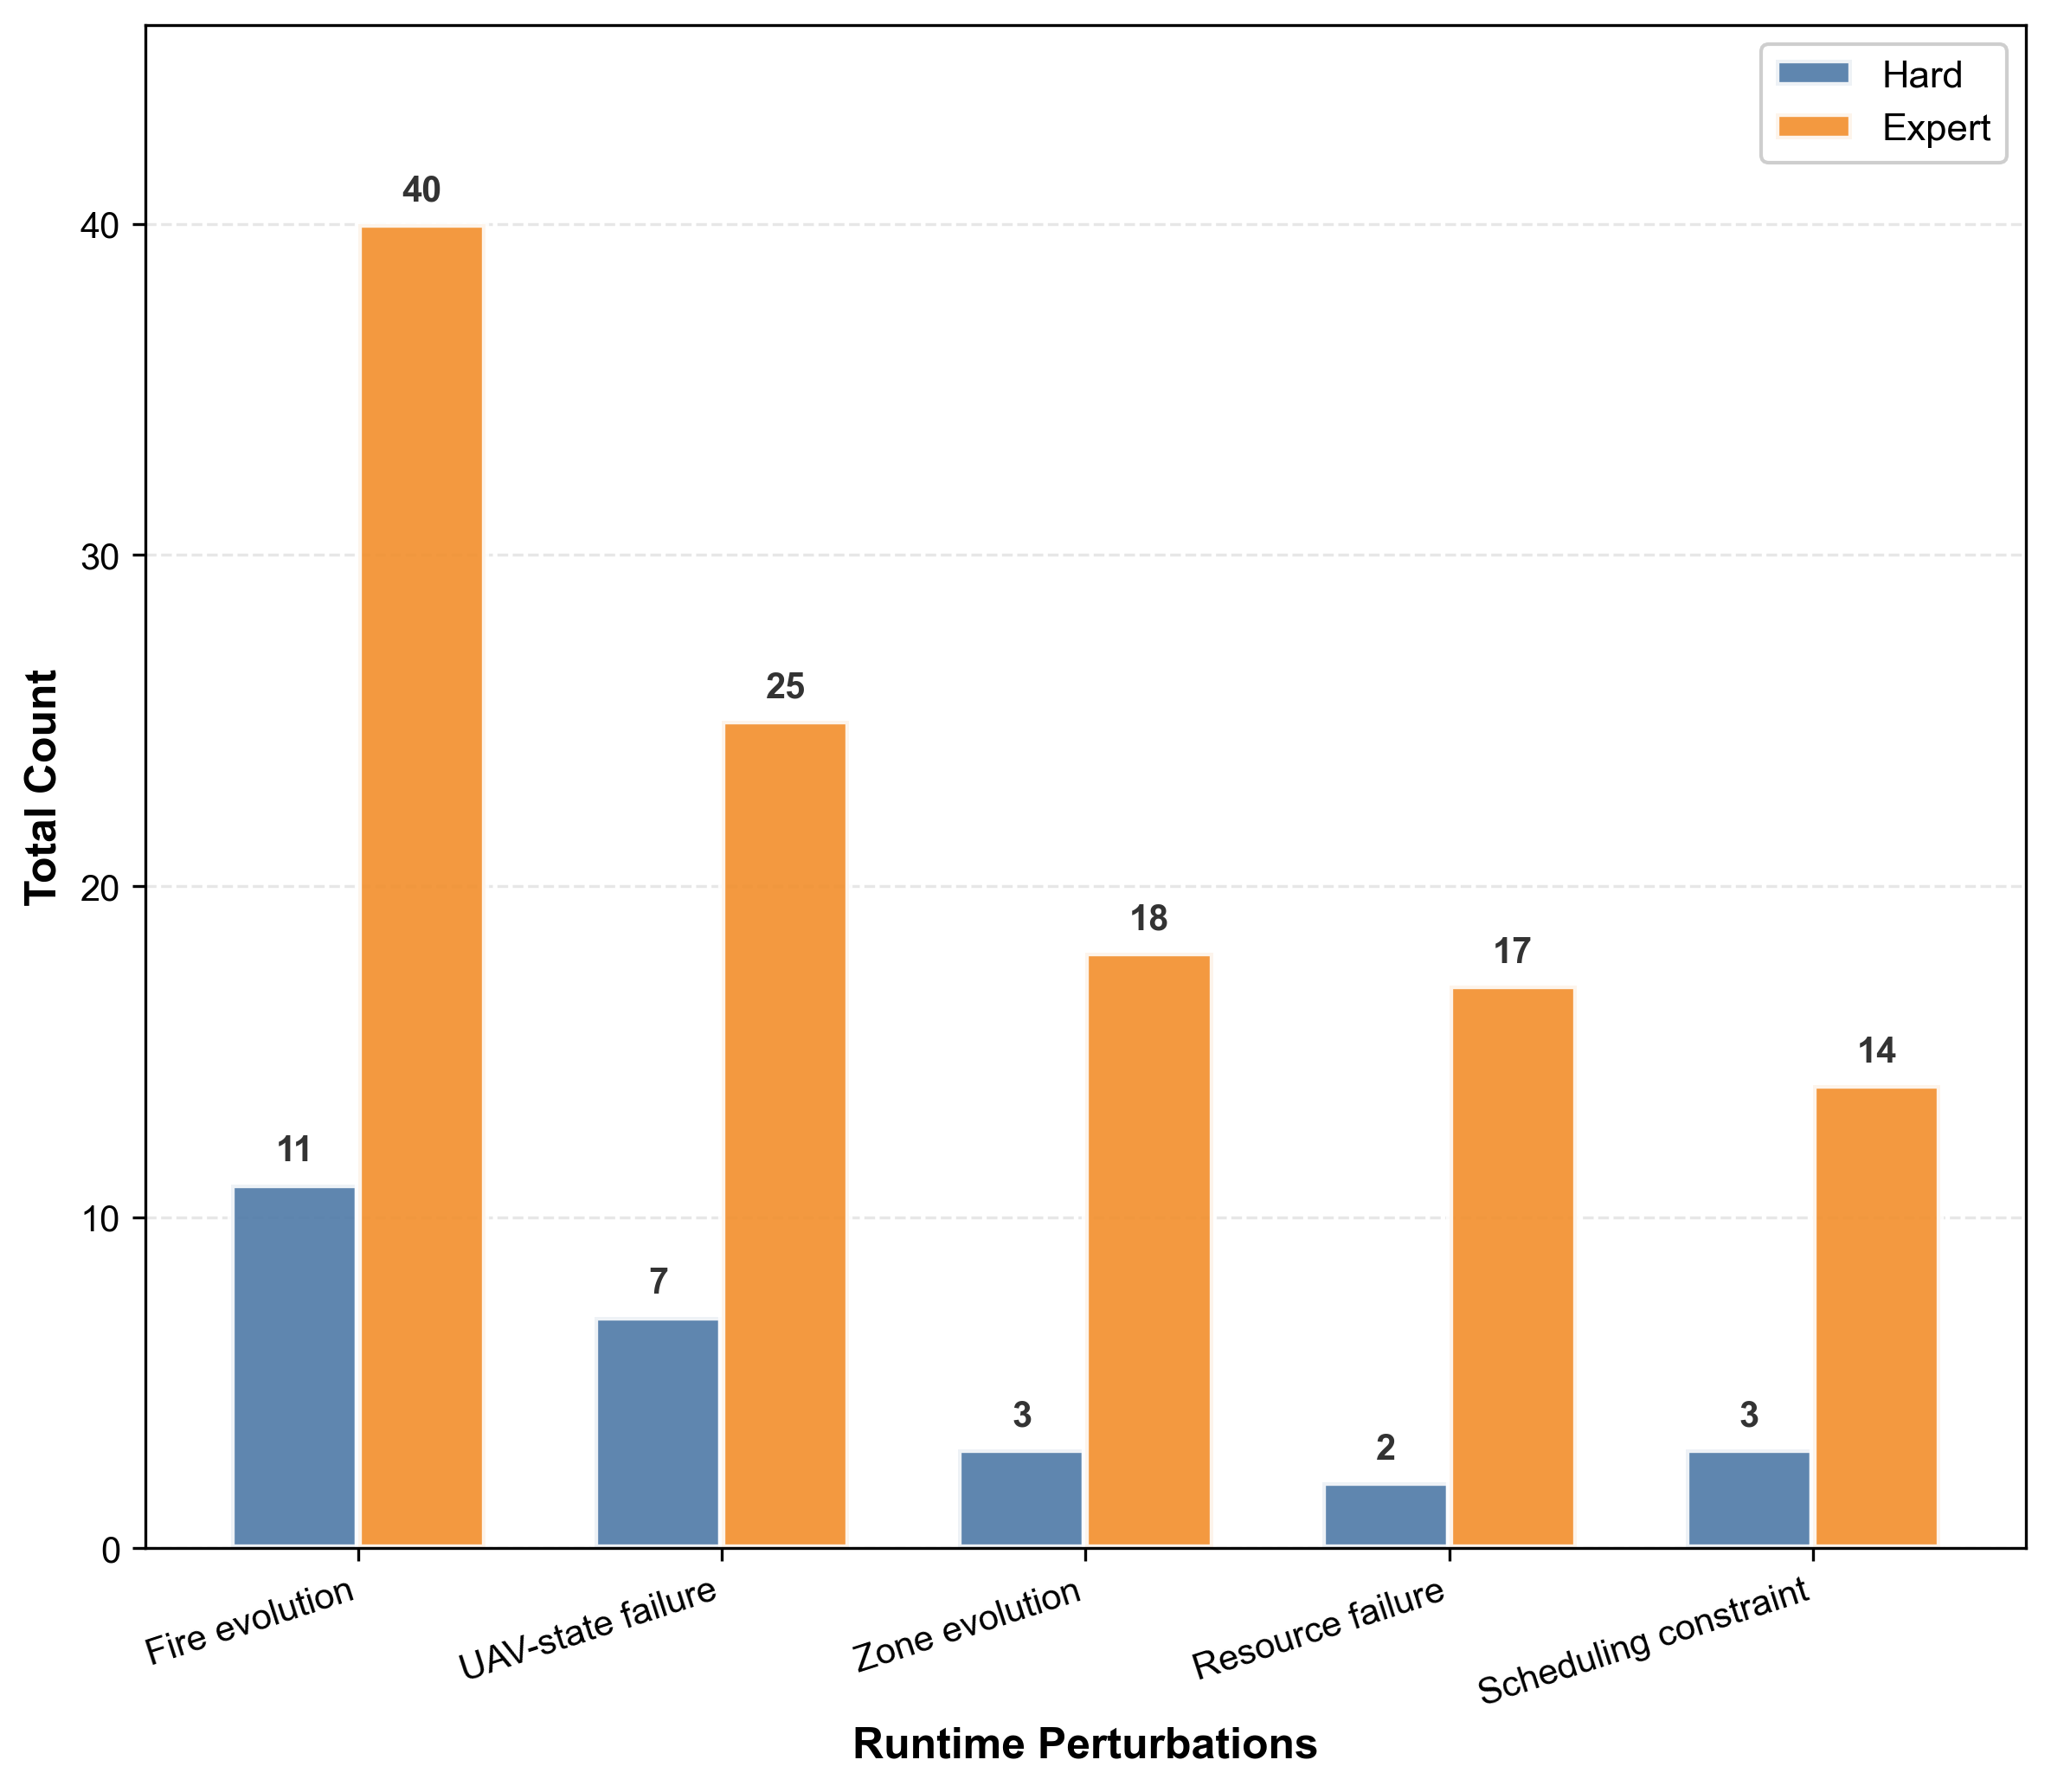
\includegraphics[width=0.35\textwidth]{figures/runtime-perturbation-sampling-distribution.png}}
    \makeatletter
    \long\def\@makecaption#1#2{%
        \@IEEEfigurecaptionsepspace
        \hbox to\hsize{\normalfont\footnotesize\hfil
            \hbox{\normalfont\footnotesize #1.\nobreakspace\nobreakspace #2}\hfil}}
    \makeatother
    \caption{Runtime perturbations used for closed-loop evaluation.}
    \label{fig:runtime-perturbation-distribution}
\end{figure*}

\subsection{Evaluation Metrics}
We evaluate end-to-end behavior using six complementary mission-level metrics:
completion, response, mission time, event stability, resource pressure, and
coordination. They measure objective attainment, response timeliness, execution
efficiency, continuity under perturbations, resource use, and workload balance,
respectively. Event stability is evaluated only in the hard and expert settings,
where runtime perturbations are introduced.

All scores are normalized to $[0,100]$, with higher values indicating better
performance. Let $Z$ be the set of task zones, $c_z\in[0,1]$ the completion
ratio of zone $z$, and $\omega_z$ its priority weight. Let
$\bar t_{\mathrm{resp}}$ and $\tau$ denote the priority-weighted mean time to
first effective intervention and the total mission duration. The six scores are
defined jointly as
\begin{equation}
\begin{aligned}
s_{\mathrm{comp}}
&=100\frac{\sum_{z\in Z}\omega_zc_z}
 {\sum_{z\in Z}\omega_z},\\
s_{\mathrm{resp}}
&=100\left[1-
\left[\frac{\bar t_{\mathrm{resp}}-l_{\mathrm{resp}}}
 {u_{\mathrm{resp}}-l_{\mathrm{resp}}}\right]_0^1\right],\\
s_{\mathrm{time}}
&=100\left[1-
\left[\frac{\tau-l_{\mathrm{time}}}
 {u_{\mathrm{time}}-l_{\mathrm{time}}}\right]_0^1\right],\\
s_{\mathrm{stab}}
&=\frac{100}{N_e}\sum_{e=1}^{N_e}
 \mathbb{I}\bigl(\mathrm{Recovered}(e)\bigr),\\
s_{\mathrm{res}}
 &=100\left[1-\frac{\bar p+\max_jp_j}{2}\right],\\
s_{\mathrm{coord}}
&=100\left[1-
\frac{G(\mathbf{n})+G(\mathbf{d})+G(\boldsymbol{\tau})}{3}\right].
\end{aligned}
\label{eq:mission-level-scores}
\end{equation}
Here, $s_{\mathrm{comp}}$, $s_{\mathrm{resp}}$, $s_{\mathrm{time}}$,
$s_{\mathrm{stab}}$, $s_{\mathrm{res}}$, and $s_{\mathrm{coord}}$ denote the
completion, response, mission time, event stability, resource pressure, and
coordination scores, respectively. $[x]_0^1=\min\{1,\max\{0,x\}\}$ clips a
value $x$ to $[0,1]$;
$l_{\mathrm{resp}}$, $u_{\mathrm{resp}}$, $l_{\mathrm{time}}$, and
$u_{\mathrm{time}}$ are fixed time-reference thresholds. $N_e$ is the number
of runtime perturbations, $e$ indexes these perturbations, and
$\mathrm{Recovered}(e)$ indicates recovery from perturbation $e$ by a feasible
revision within the allowed window. $\mathbb{I}(\cdot)$ is the
indicator function, which equals 1 when its condition is true and 0 otherwise.
$p_j\in[0,1]$ and $\bar p$ denote the resource pressure of UAV $j$ and the
fleet-average resource pressure, respectively, where $j$ indexes the UAVs in
the fleet. $G(\cdot)\in[0,1]$ is the Gini coefficient of the assigned task
counts $\mathbf{n}$, flight distances $\mathbf{d}$, or execution durations
$\boldsymbol{\tau}$.

Because no perturbations are introduced in the simple and normal settings,
their applicable metric set $\mathcal{K}_d$ contains completion, response,
mission time, resource pressure, and coordination; for the hard and expert
settings, it additionally contains event stability.
For each episode $i$ at difficulty level $d$, the score combines the weighted
aggregation of its applicable metrics with a bounded difficulty reward. The
reported score for level $d$ is the mean across its $N_d$ episodes:
\begin{equation}
\begin{aligned}
S_d
&=\frac{1}{N_d}\sum_{i=1}^{N_d}
\left[\sum_{k\in\mathcal{K}_d}w_{k,d}s_{i,k}
\frac{1+\lambda\rho_i}{1+\lambda}\right],\\
w_{k,d}&\geq0,\qquad
\sum_{k\in\mathcal{K}_d}w_{k,d}=1.
\end{aligned}
\label{eq:final-evaluation-score}
\end{equation}
Here, $s_{i,k}$ is the score of episode $i$ for metric $k$, and $w_{k,d}$
is its normalized weight at difficulty level $d$. The coefficient
$\rho_i\in[0,1]$ represents episode difficulty, while $\lambda\geq0$ controls
the difficulty reward; division by $1+\lambda$ keeps $S_d$ within $[0,100]$.
The component scores support diagnostic analysis, whereas $S_d$ provides the
overall comparison score for level $d$.

Together, the staged episode difficulty and decomposed metrics provide a common
basis for testing the three questions examined next: whether CLoMA-UWR sustains
high-level closed-loop decision making, which mechanisms
matter as operational pressure increases, and how much capability for
resource-constrained mission planning can be retained by a compact planner.

\endinput

% !TEX root = ../main.tex
\section{Experiments}
\label{sec:experiments}

This section evaluates CLoMC-UWR with the evaluation suite in
Section~\ref{sec:evaluation-suite} through three settings. The first examines
whether CLoMC-UWR outperforms an Optimization-Based Planner as
operational pressure increases and how sensitive it is to model choice. The
second isolates how Validation, Memory, and Runtime Replanning address their
respective decision risks, while the third tests whether validated
demonstrations can specialize a compact planner with lower planning overhead.
The following subsections specify the experimental setup and then report the
end-to-end, ablation, and fine-tuned planner evaluations.

\subsection{Experimental Setup}

\subsubsection{End-to-End Setting}
We fix Gemini~3.1~Pro for Vision Analysis and use ChatGPT~5.5,
Gemini~3.1~Pro, Claude~Opus~4.7, or DeepSeek~V4~Pro in Mission Planning,
Validation, and Runtime Replanning. Fixing Vision Analysis keeps the
structured fire situation consistent, so differences among the four downstream
foundation-model configurations reflect the downstream decision process.

The Optimization-Based Planner is implemented with the CP-SAT solver in Google
OR-Tools. It shares the Vision Analysis output, UAV operational states, mission constraints,
and action space with CLoMC-UWR, and re-optimizes the remaining
task chains from the updated operational state after each runtime perturbation.
Its downstream decision process does not use an LLM, Validation, or Memory. The
baseline and four foundation-model configurations use the same 80 episodes---20
at each difficulty level---and the same execution and scoring procedure.

\subsubsection{Ablation Setting}
Using the DeepSeek~V4~Pro configuration, we compare CLoMC-UWR with w/o
Validation, w/o Memory, and w/o Runtime Replanning. These variants respectively
remove Validation, disable retrieval from Memory, and retain the initial plan
after runtime perturbations. All other models, prompts, and execution settings
remain unchanged, and all four configurations use the same 80 episodes, with 20
at each difficulty level.
Because simple and normal episodes contain no runtime perturbations, Runtime
Replanning remains inactive; the w/o Runtime Replanning variant therefore
introduces no other execution difference at these levels.

\subsubsection{Fine-Tuning Data and Training}
We construct 2,000 mission-planning demonstrations using CLoMC-UWR
with Gemini~3.1~Pro as the teacher planner from mission situations disjoint from
the 80 evaluation episodes. Each demonstration maps $(\mathcal{Z},U,C)$ to $P$, pairing
the task zones, UAV operational states, and mission constraints with the final multi-UAV
plan accepted by Validation. These validated demonstrations specialize
Qwen3-8B for the planning mapping in Section~\ref{sec:system-design}. We use a
90\%/10\%
training/validation split and 4-bit quantized low-rank adaptation with a maximum
sequence length of 6,144 tokens, three epochs, an effective batch size of 16,
and a learning rate of $5\times10^{-5}$. Fine-tuning uses one NVIDIA GeForce
RTX~4090, 16 Intel Xeon Gold~6430 vCPUs, and 120~GB of system memory.

\subsubsection{Planner Evaluation Protocol}
We evaluate the original and fine-tuned Qwen3-8B by replacing only the planner
used by Mission Planning. Vision Analysis and Validation retain
Gemini~3.1~Pro, while all non-LLM components remain unchanged. Both
configurations use the same 40 simple and normal episodes---20 at each
level---from the first setting. Because these episodes
contain no runtime perturbations, the experiment neither invokes Runtime
Replanning nor assesses event stability, thereby isolating planner fine-tuning.

\subsection{End-to-End Evaluation}

Table~\ref{tab:main-results} reports the end-to-end results, while
Figures~\ref{fig:model-total-score} and~\ref{fig:model-performance-radar}
summarize the overall scores and mission-level profiles.

\begin{figure}[!t]
    \centering
    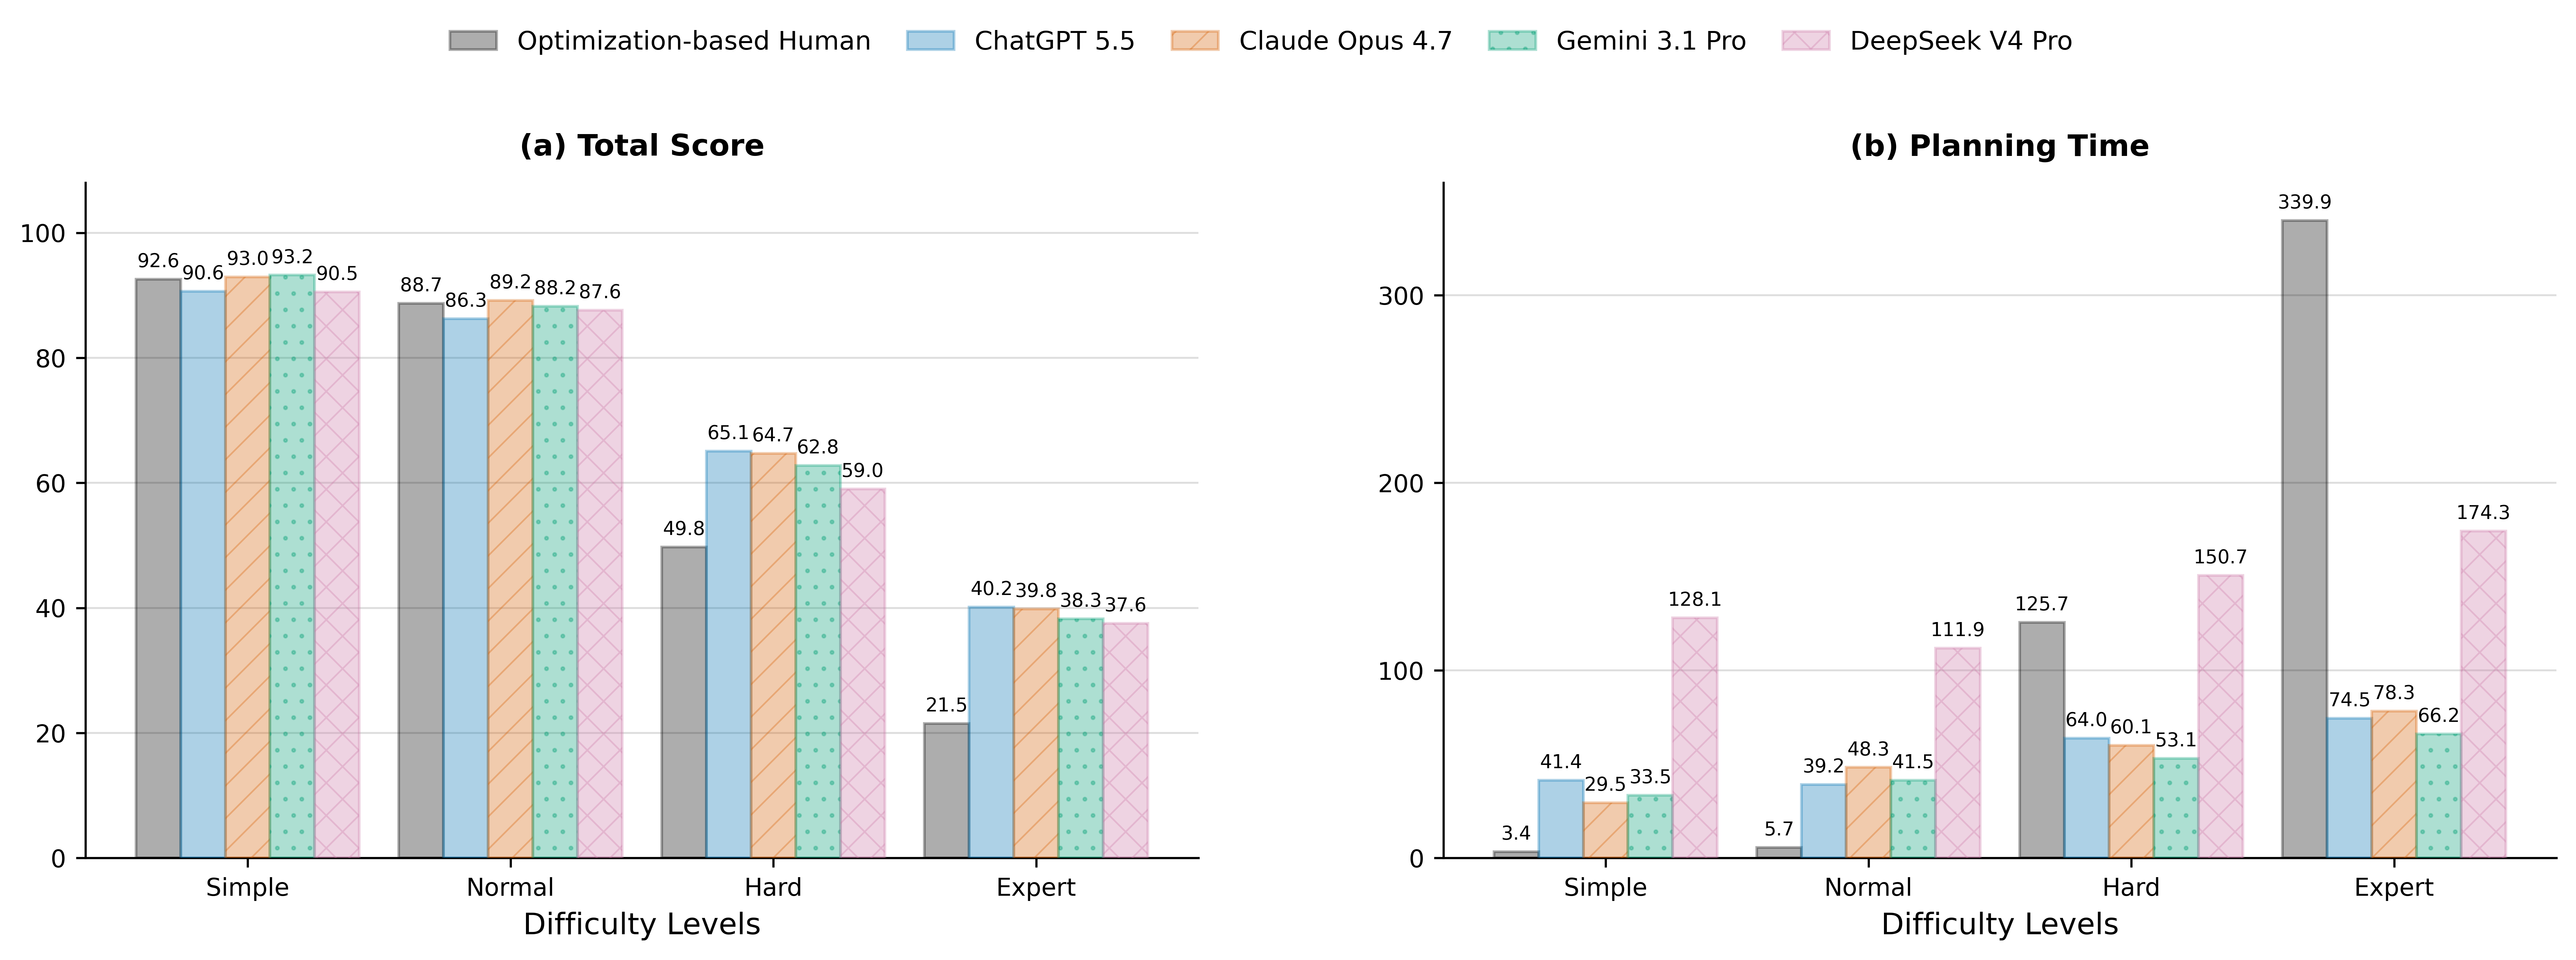
\includegraphics[width=\columnwidth]{figures/foundation-model-overall-scores.png}
    \caption{Overall scores of the Optimization-Based Planner and four
    foundation-model configurations across episode difficulty levels.}
    \label{fig:model-total-score}
\end{figure}

\begin{table*}[!t]
    \centering
    \caption{End-to-end results for the Optimization-Based Planner and the
    proposed framework across episode difficulty levels. Optimization-Based
    denotes the Optimization-Based Planner, while each model name denotes the
    corresponding downstream foundation-model configuration of the proposed
    framework.
    $S$ is the overall score, and the remaining columns report normalized mission-level scores in
    $[0,100]$ (higher is better). Event stability is not applicable to the
    simple and normal settings and is denoted by ``--''. The highest observed
    value for each metric at every difficulty level is shown in bold when it is
    unique; these highlights describe the evaluated configurations rather than
    a general ranking of foundation models.}
    \label{tab:main-results}
    \footnotesize
    \setlength{\tabcolsep}{1.5pt}
    \renewcommand{\arraystretch}{1.12}
    \begin{tabular*}{\textwidth}{@{\extracolsep{\fill}}llcrrrrrr@{}}
        \toprule
        \multirow{2}{*}{\textbf{Difficulty}}
        & \multirow{2}{*}{\textbf{Configuration}}
        & \multirow{2}{*}{\textbf{$S$}}
        & \multicolumn{6}{c}{\textbf{Mission-level score}} \\
        \cmidrule(l){4-9}
        & &
        & \textbf{Completion}
        & \textbf{Response}
        & \textbf{Time}
        & \makecell{\textbf{Event}\\\textbf{stability}}
        & \makecell{\textbf{Resource}\\\textbf{pressure}}
        & \textbf{Coordination} \\
        \midrule

        Simple & Optimization-Based
        & 92.59 & 100.00 & \textbf{92.34} & 88.94
        & -- & \textbf{85.64} & 82.31 \\
        & ChatGPT~5.5
        & 90.63 & 100.00 & 89.18 & 78.99
        & -- & 81.20 & 79.54 \\
        & Gemini~3.1~Pro
        & \textbf{93.23} & 100.00 & 88.78 & \textbf{91.06} & -- & 84.45 & 80.71 \\
        & Claude~Opus~4.7
        & 92.97 & 100.00 & 91.44 & 86.62 & -- & 82.18 & \textbf{83.96} \\
        & DeepSeek~V4~Pro
        & 90.54 & 100.00 & 87.66 & 78.90 & -- & 83.05 & 80.04 \\
        \addlinespace

        Normal & Optimization-Based
        & 88.72 & 100.00 & 89.07 & \textbf{72.71}
        & -- & \textbf{87.05} & 77.74 \\
        & ChatGPT~5.5
        & 86.28 & 100.00 & 93.82 & 66.27
        & -- & 77.64 & 73.19 \\
        & Gemini~3.1~Pro
        & 88.23 & 100.00 & 94.10 & 71.50 & -- & 86.68 & 71.72 \\
        & Claude~Opus~4.7
        & \textbf{89.18} & 100.00 & \textbf{96.09} & 68.24 & -- & 84.54 & \textbf{78.12} \\
        & DeepSeek~V4~Pro
        & 87.63 & 100.00 & 91.36 & 71.74 & -- & 83.95 & 75.13 \\
        \addlinespace

        Hard & Optimization-Based
        & 49.77 & 96.40 & 78.32 & 26.94
        & 20.75 & 54.86 & 52.14 \\
        & ChatGPT~5.5
        & \textbf{65.09} & 100.00 & \textbf{94.97} & \textbf{41.22}
        & \textbf{42.25} & \textbf{63.19} & \textbf{67.24} \\
        & Gemini~3.1~Pro
        & 62.81 & 100.00 & 92.58 & 39.60 & 33.75 & 59.10 & 60.65 \\
        & Claude~Opus~4.7
        & 64.74 & 99.86 & 94.22 & 35.28 & 40.50 & 62.15 & 65.88 \\
        & DeepSeek~V4~Pro
        & 59.03 & 98.57 & 83.90 & 30.76 & 34.75 & 61.36 & 59.07 \\
        \addlinespace

        Expert & Optimization-Based
        & 21.53 & 78.27 & 42.13 & 1.93
        & 0.00 & 42.07 & 39.87 \\
        & ChatGPT~5.5
        & \textbf{40.15} & \textbf{93.24} & \textbf{67.01} & \textbf{13.23}
        & \textbf{2.67} & \textbf{60.15} & \textbf{61.25} \\
        & Gemini~3.1~Pro
        & 38.28 & 90.09 & 61.30 & 12.02 & 0.00 & 58.72 & 55.82 \\
        & Claude~Opus~4.7
        & 39.81 & 92.43 & 65.55 & 9.13 & 0.00 & 58.99 & 60.11 \\
        & DeepSeek~V4~Pro
        & 37.55 & 90.95 & 61.09 & 3.54 & 0.00 & 53.43 & 54.43 \\
        \bottomrule
    \end{tabular*}
\end{table*}


In the simple and normal settings, where no runtime perturbations occur, all
evaluated methods achieve complete task coverage. The Optimization-Based
Planner obtains overall scores of 92.59 and 88.72, respectively, which lie
within the corresponding ranges of the four foundation-model configurations
(90.54--93.23 and 86.28--89.18), confirming that it remains competitive under
lower operational pressure.

Once runtime perturbations are introduced, the difference between the two
decision approaches becomes more pronounced: the Optimization-Based Planner
scores 49.77 and 21.53 in the hard and expert settings, respectively 9.26 and
16.02 points below the lowest-scoring foundation-model configuration. Its expert
completion score is 78.27, compared with 90.09--93.24 for the four
configurations. Because its event stability score of 0 overlaps their 0--2.67
range, the advantage of CLoMC-UWR also reflects task completion
and the other execution-quality metrics.

\begin{figure}[!htbp]
    \centering
    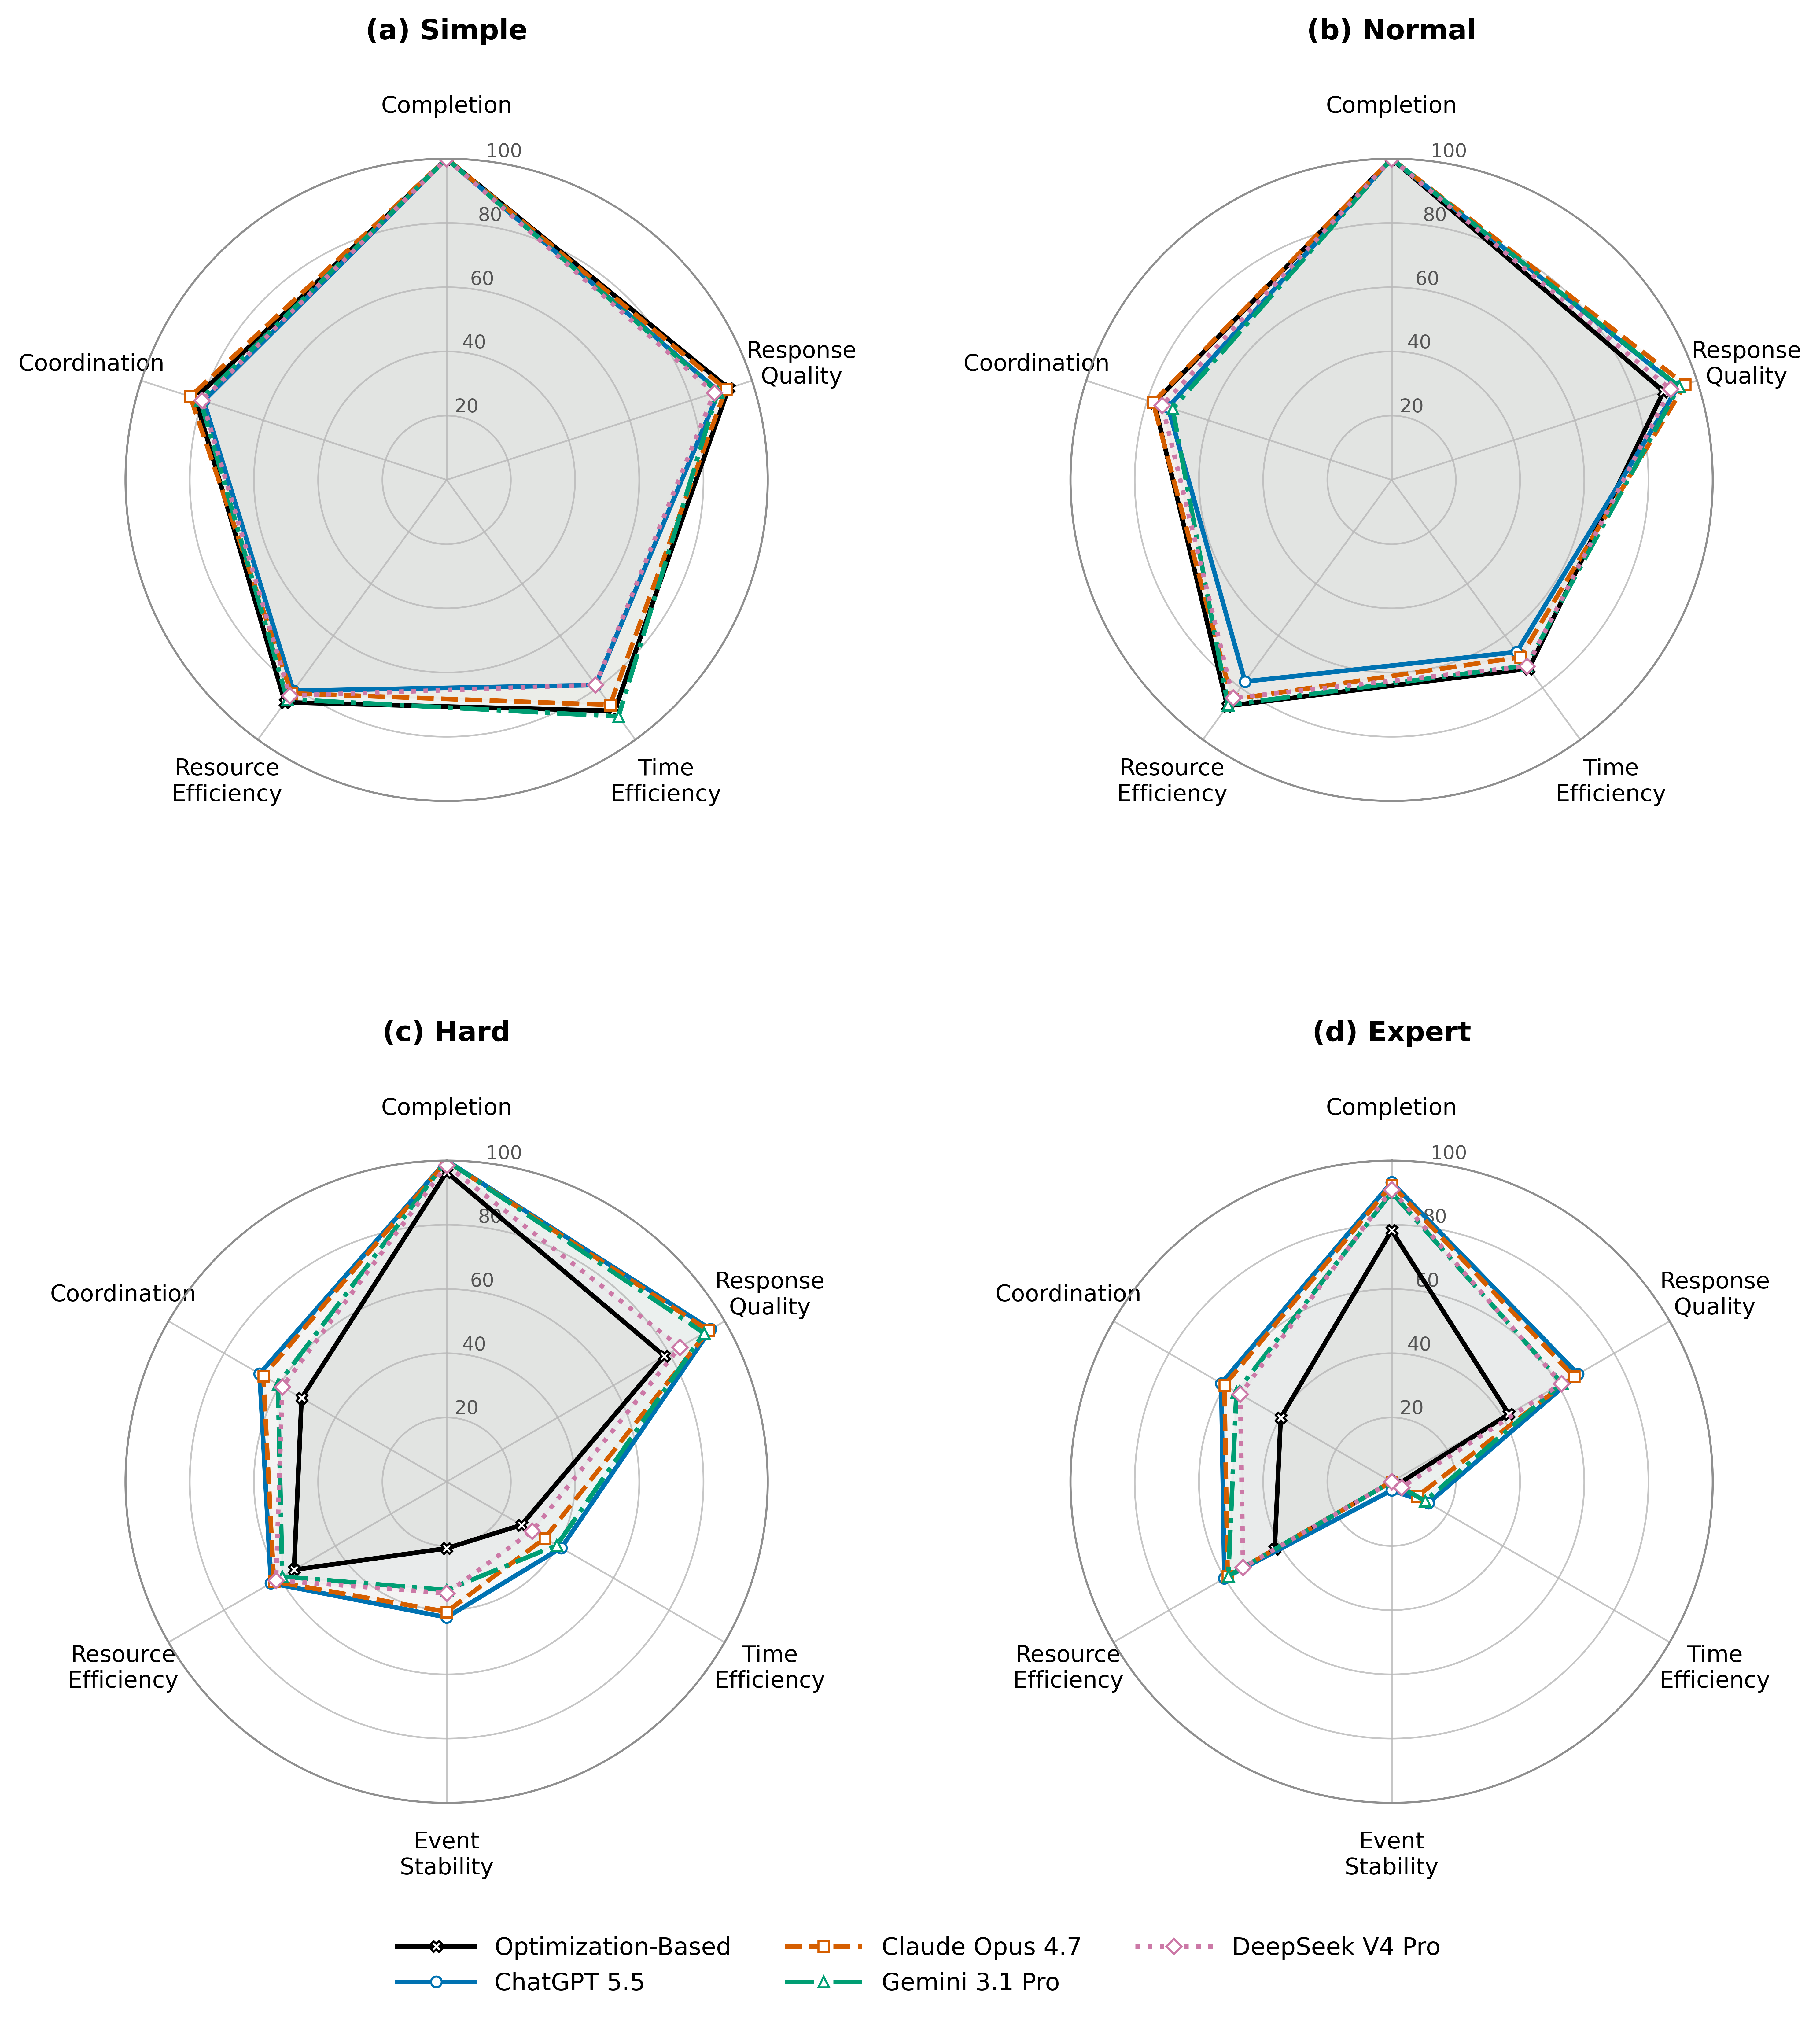
\includegraphics[width=0.95\columnwidth]{figures/foundation-model-performance-radar.png}
    \caption{Mission-level performance profiles of the Optimization-Based
    Planner and four foundation-model configurations at each difficulty level.
    Larger radial values indicate better performance.}
    \label{fig:model-performance-radar}
\end{figure}

Among the four foundation-model configurations, Gemini~3.1~Pro obtains the
highest overall score in the simple setting, Claude~Opus~4.7 in the normal
setting, and ChatGPT~5.5 in the hard and expert settings. Because this ordering
changes with difficulty, the results do not yield a single model ranking. All
four configurations maintain high basic task completion in the hard and expert
episodes, but their mission time scores fall to 3.54--13.23 and their event
stability scores to 0--2.67 under expert conditions. Model choice thus
affects the downstream decision process, but changing the foundation model
alone does not prevent the common degradation as operational pressure
increases.

Taken together, the Optimization-Based Planner remains competitive in the
simple and normal episodes, where no runtime perturbations occur. Under the
higher operational pressure of the hard and expert episodes, CLoMC-UWR
maintains higher basic task completion and execution quality across
all four downstream foundation-model configurations. The common decline in
mission time and event stability under expert conditions nevertheless leaves
clear headroom for more robust replanning and time-aware resource allocation.

\subsection{Ablation Studies}

Table~\ref{tab:ablation-results} reports the ablation results with
DeepSeek~V4~Pro fixed as the foundation model. Removing Validation causes a
modest but consistent reduction across all four difficulty levels, with drops
of 2.16, 2.33, 3.81, and 2.05 points from simple to expert. The limited change
in average mission score does not imply that the module remains inactive: the
validation loop is triggered 5, 5, 4, and 6 times in the simple, normal, hard,
and expert settings, respectively. These interventions suggest that Validation
primarily serves as an occasional reliability safeguard against invalid or
tactically implausible plans rather than as a continuous source of score
improvement.

\begin{table}[!htbp]
    \centering
    \caption{Ablation results with DeepSeek~V4~Pro as the foundation model.
    Values report the mean overall score $S$ over 20 episodes at each
    difficulty level. The best result in each column is shown in bold.}
    \label{tab:ablation-results}
    \small
    \setlength{\tabcolsep}{7pt}
    \renewcommand{\arraystretch}{1.15}
    \begin{tabular}{@{}lcccc@{}}
        \toprule
        \multirow{2}{*}{\textbf{Configuration}}
        & \multicolumn{4}{c}{\textbf{Overall score $S$}} \\
        \cmidrule(l){2-5}
        & \textbf{Simple} & \textbf{Normal} & \textbf{Hard} & \textbf{Expert} \\
        \midrule
        Full
        & \textbf{90.54} & 87.63 & \textbf{59.03} & \textbf{37.55} \\
        w/o Validation
        & 88.38 & 85.30 & 55.22 & 35.50 \\
        w/o Memory
        & 88.57 & 86.94 & 49.35 & 22.10 \\
        w/o Runtime Replanning
        & 90.33 & \textbf{88.14} & 35.86 & 12.98 \\
        \bottomrule
    \end{tabular}
\end{table}


Figure~\ref{fig:ablation-score-delta} visualizes the score change of each
ablated variant relative to CLoMC-UWR.

\begin{figure}[!t]
    \centering
    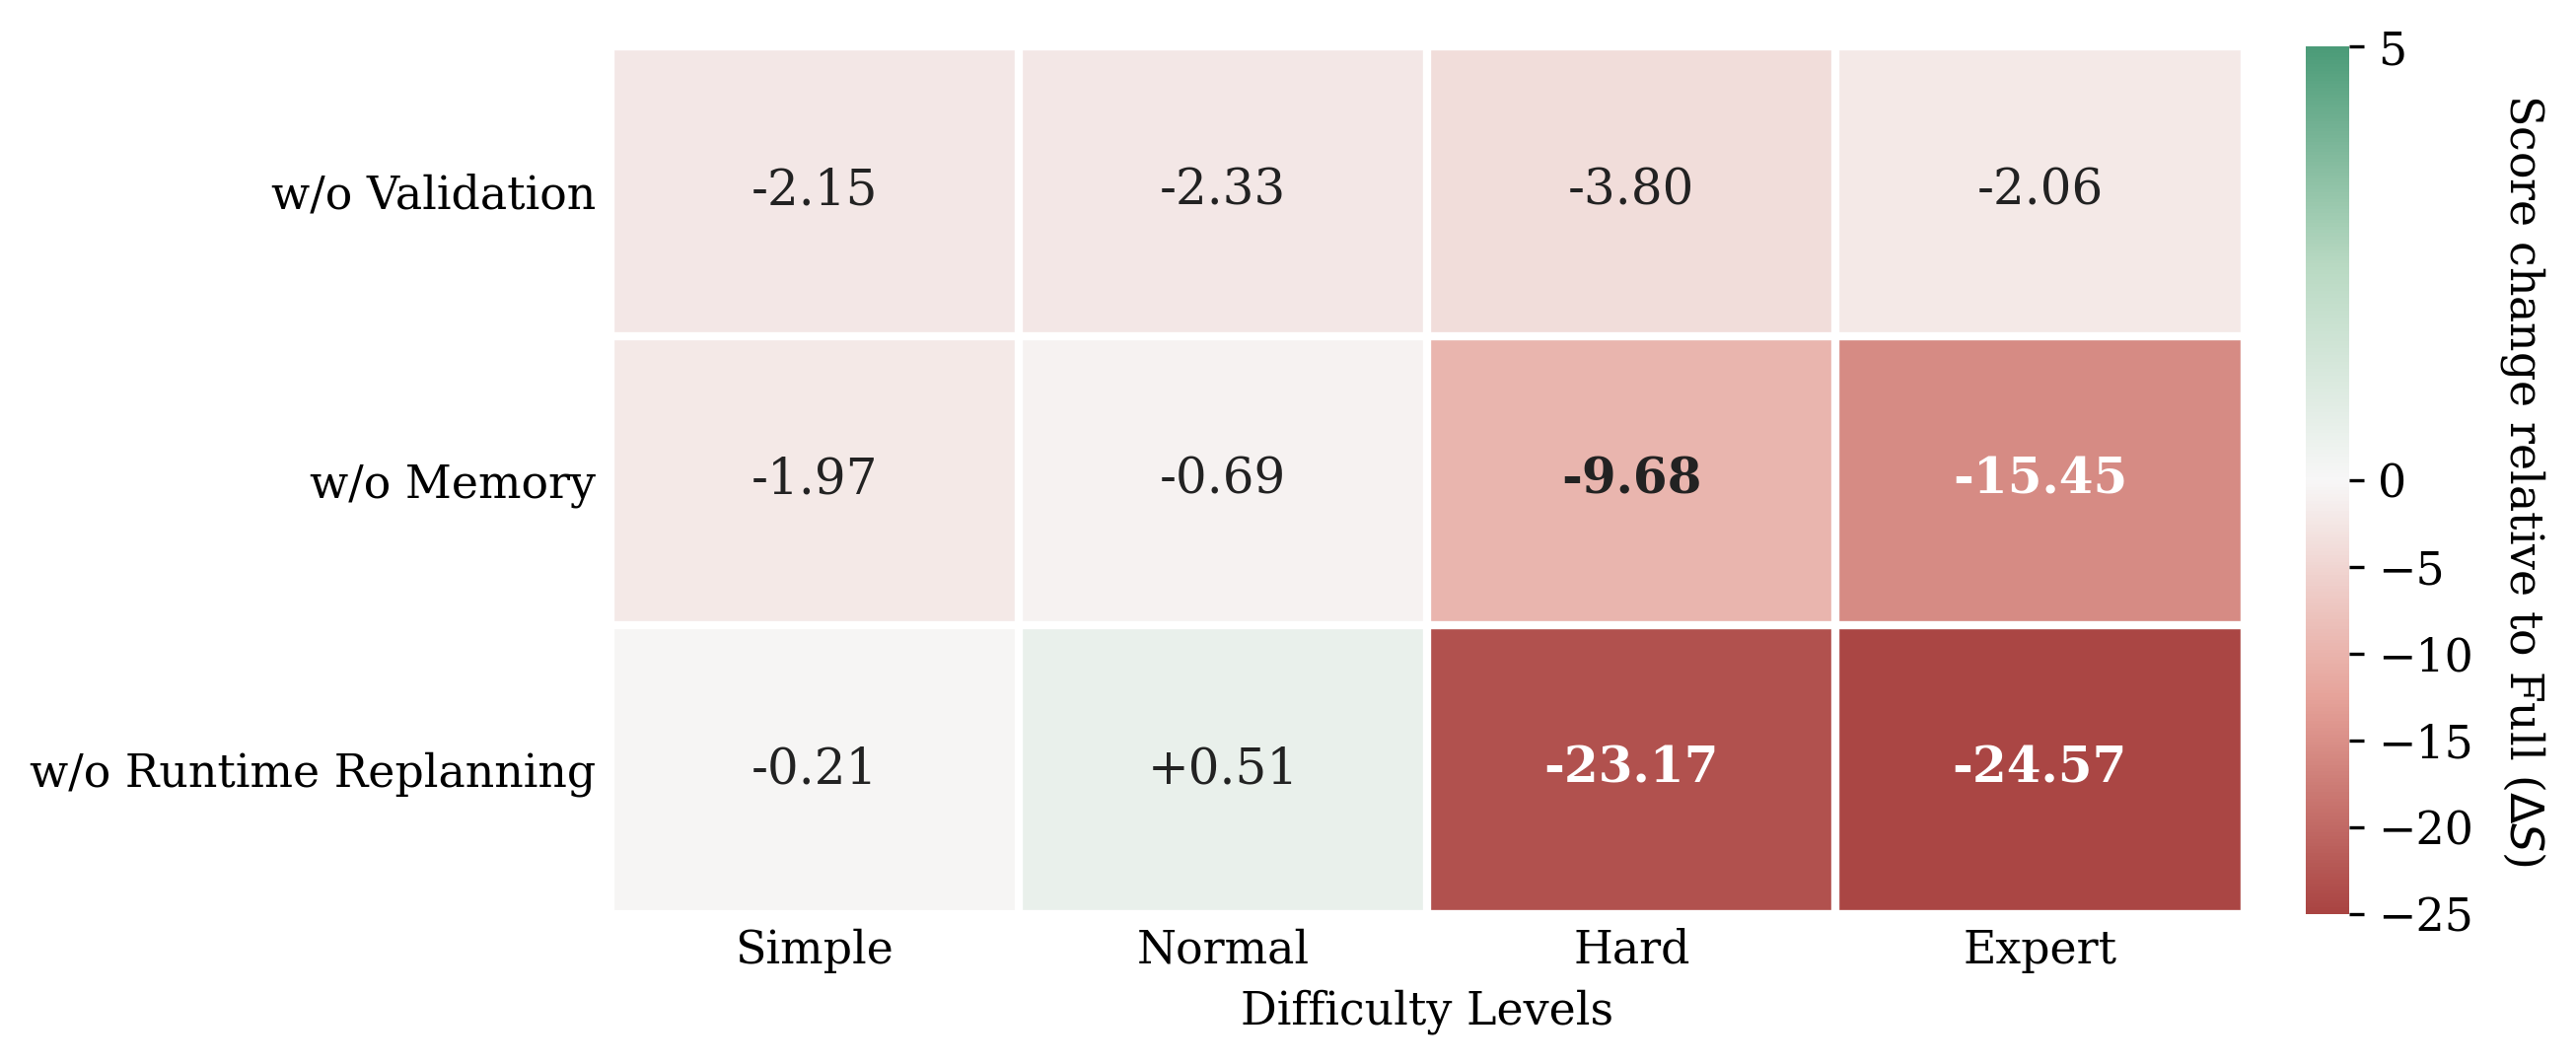
\includegraphics[width=\columnwidth]{figures/ablation-score-change-heatmap.png}
    \caption{Change in overall score relative to CLoMC-UWR for each ablated
    variant and difficulty level. Negative values indicate performance
    degradation, while positive values indicate improvement.}
    \label{fig:ablation-score-delta}
\end{figure}

The contribution of Memory becomes more pronounced as operational pressure
increases.
Removing Memory reduces the score by only 1.97 points in the
simple setting and 0.69 points in the normal setting, but the reduction grows
to 9.68 points in hard episodes and 15.45 points in expert episodes. This
pattern indicates that retrieved task situations, plans, and outcomes are most useful
when resource constraints, event interactions, and scheduling pressure make
planning less routine.

Disabling Runtime Replanning has little effect in the simple and normal
settings, where no perturbations are triggered. In contrast, its score falls
from 59.03 to 35.86 in hard episodes and from 37.55 to 12.98 in expert
episodes. The sharp degradation confirms that an initially valid plan is
insufficient once the execution state changes, and that Runtime Replanning is
the key mechanism for maintaining mission performance under perturbations.

The ablations therefore do not indicate three mechanisms that contribute
uniformly in every episode. Validation acts as a low-frequency safeguard
against invalid candidate plans, Memory contributes most when operational
pressure makes planning less routine, and Runtime Replanning becomes critical
when runtime perturbations invalidate an accepted plan. Their condition-dependent
effects explain why all three are retained in CLoMC-UWR despite
their different average score contributions.

\subsection{Fine-Tuned Planner Evaluation}

\begin{figure}[!t]
    \centering
    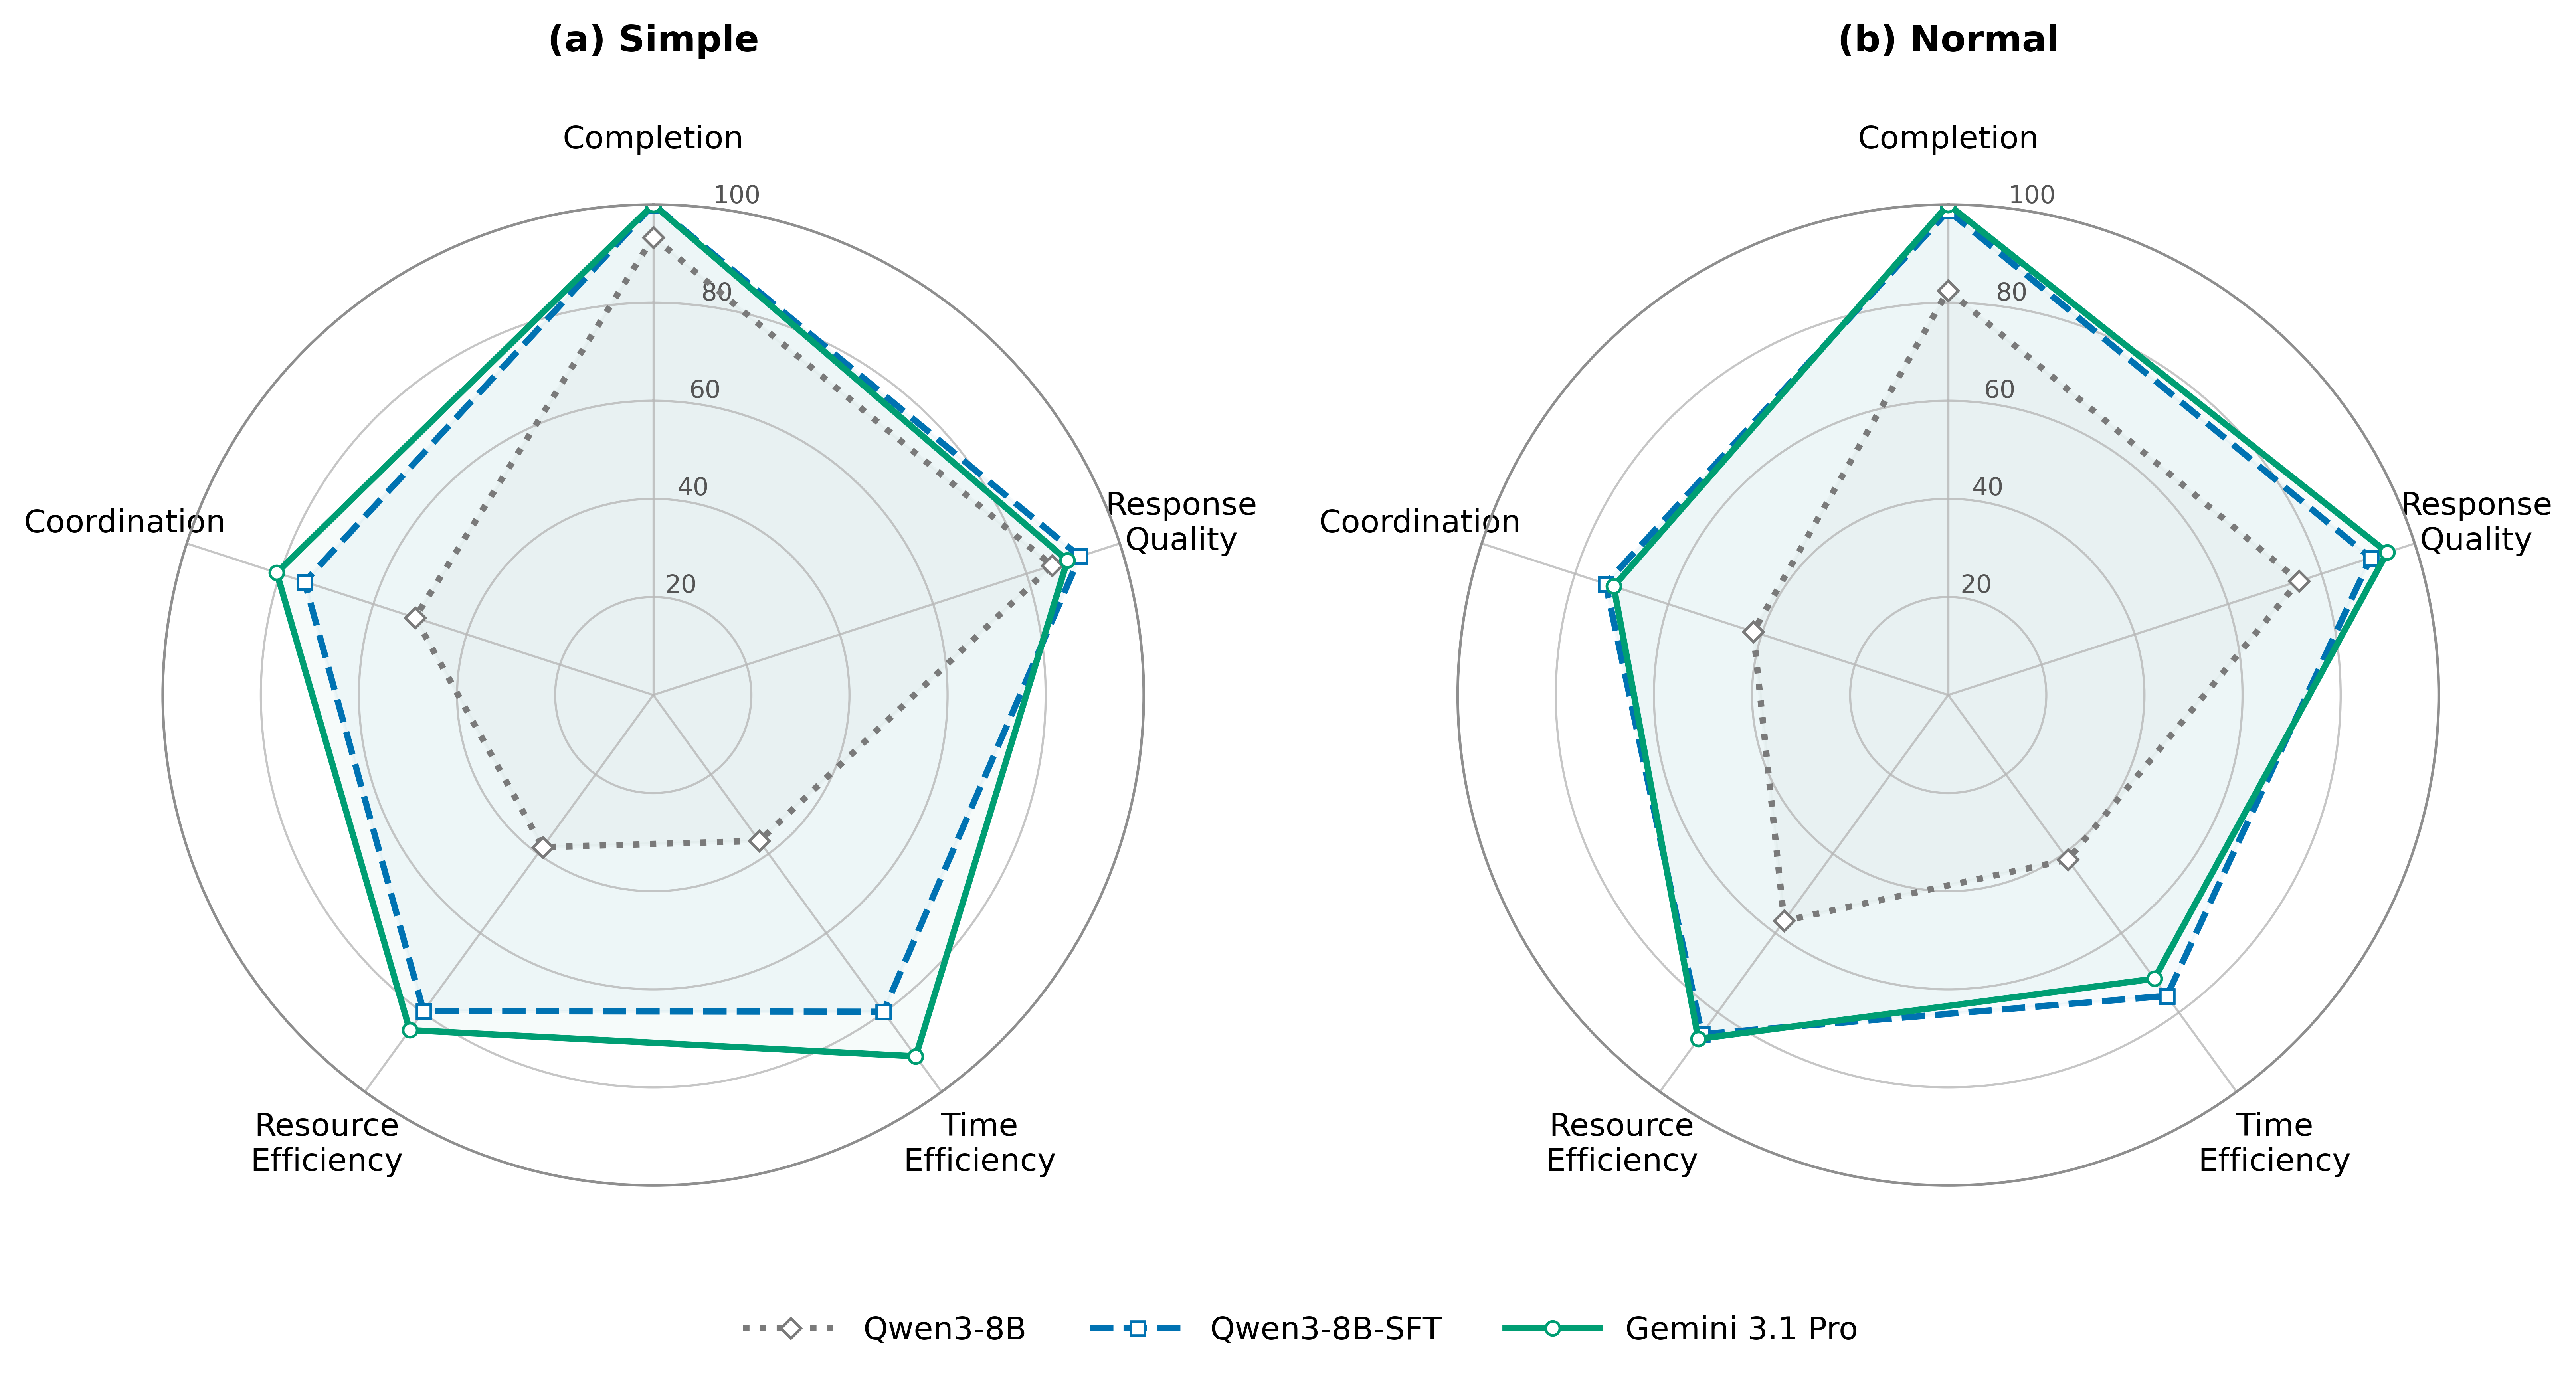
\includegraphics[width=\columnwidth]{figures/planner-performance-radar.png}
    \caption{Mission-level profiles of the three planners in the simple and
    normal settings. Larger radial values indicate better performance. Event
    stability is not interpreted because neither setting contains runtime
    perturbations.}
    \label{fig:planner-performance-radar}
\end{figure}

\begin{figure*}[!b]
    \centering
    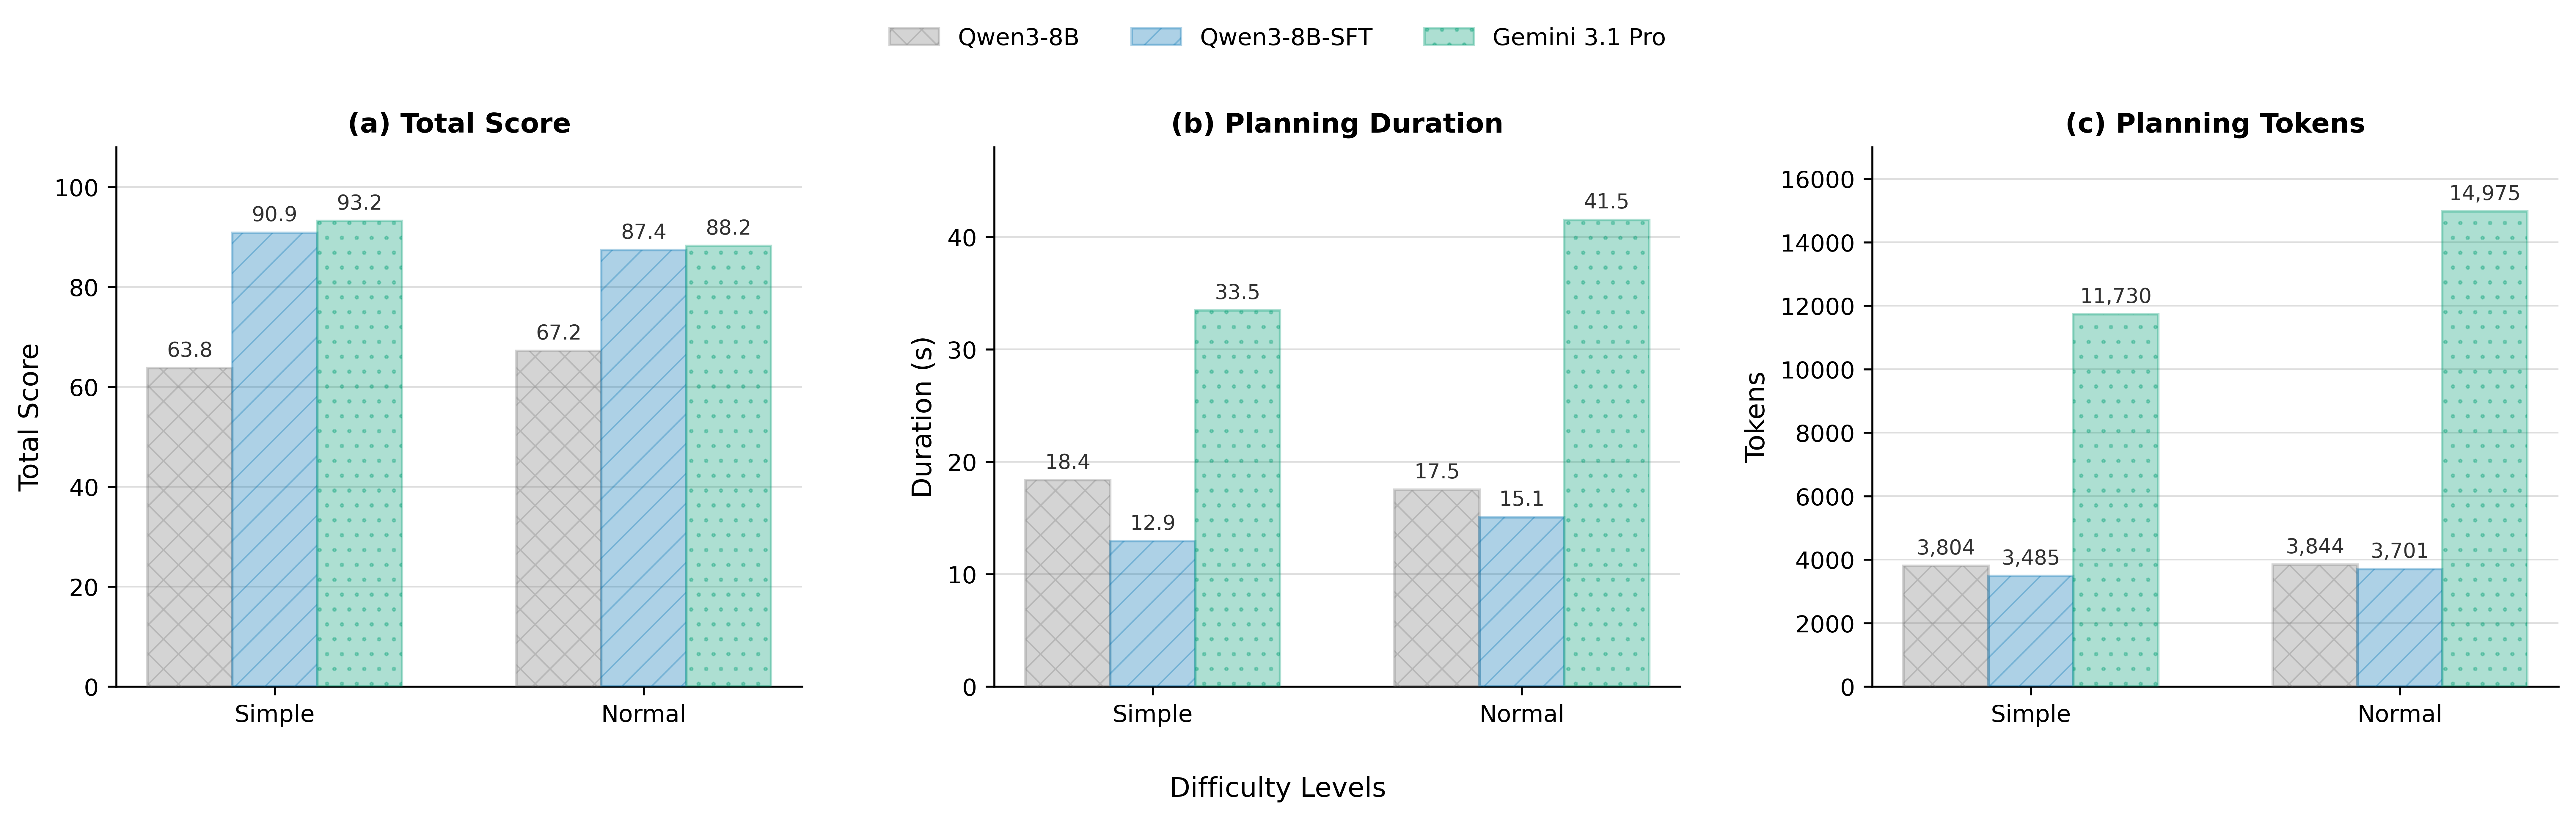
\includegraphics[width=\textwidth]{figures/planner-score-efficiency-comparison.png}
    \caption{Score--efficiency comparison of the three planners: (a) total
    score, (b) planning duration, and (c) planning-token usage. Lower values are
    better in (b) and (c).}
    \label{fig:planner-score-efficiency}
\end{figure*}

Table~\ref{tab:fine-tuned-planner-results} compares the Gemini~3.1~Pro
teacher planner with the original and fine-tuned Qwen3-8B planners. Fine-tuning
substantially improves the compact planner on both difficulty levels, yielding
an average absolute gain of 23.65 points and reaching 98.24\% of the
Gemini~3.1~Pro teacher planner's average score across the simple and normal
settings.

\input{tables/planner-fine-tuning-results}

Figure~\ref{fig:planner-performance-radar} shows that the improvement extends
across the mission-level performance profile. The original Qwen3-8B exhibits
its largest deficits in mission time, resource pressure, and coordination,
whereas fine-tuning substantially expands its profile toward that of
Gemini~3.1~Pro. The fine-tuned planner restores near-complete task coverage and
slightly exceeds Gemini~3.1~Pro in simple-level response and normal-level
mission time and coordination. This indicates that the validated demonstrations
transfer not only output-format compliance but also task-allocation and
resource-management behavior to the compact planner.

The fine-tuned planner also reduces planning overhead under the evaluated
deployment setting. Its mean planning time across the two levels is 14.01~s,
compared with 37.50~s for Gemini~3.1~Pro, while its mean planning-token usage
falls from 13,353 to 3,593. Figure~\ref{fig:planner-score-efficiency} summarizes
this performance--efficiency trade-off. This evidence is limited to initial
planning on the evaluated simple and normal episodes; it does not establish how
the compact planner would perform with Runtime Replanning under hard or expert
conditions.

\FloatBarrier

\endinput

% !TEX root = ../main.tex
\section{Conclusion}

Within the task and evaluation setting studied here, the results support the
use of LLMs as the high-level closed-loop decision core of a
resource-constrained multi-UAV wildfire rescue system. This capability is not
uniformly robust: the complete decision loop remains effective in terms of
basic task completion, but execution quality and mission continuity deteriorate
as operational pressure increases. The proposed LLM-centered closed-loop
decision framework addresses this problem by connecting fire-situation
understanding and resource-constrained mission planning with Validation,
Memory, and Runtime Replanning.

Three sets of evidence support this conclusion. First, the Optimization-Based
Planner remains competitive in the simple and normal episodes, whereas the
complete framework maintains higher basic task completion and execution quality
in the hard and expert episodes across four downstream foundation-model
configurations. This also shows that end-to-end operation is not confined to
one downstream model, although all four configurations lose execution quality
under greater operational pressure. Second, the ablations show condition-dependent
roles: Validation provides an occasional reliability safeguard, Memory becomes
increasingly valuable as resource and scheduling interactions intensify, and
Runtime Replanning is critical when perturbations invalidate an active plan.
Third, Qwen3-8B fine-tuned with validated planning demonstrations retains
98.24\% of the Gemini~3.1~Pro teacher planner's average score on simple and
normal episodes, while reducing mean planning time by approximately 63\% and
planning-token usage by 73\%. This final result supports lower-cost local
deployment of Mission Planning within the evaluated setting.

This answer remains limited to a calibrated simulation, a fixed
episode set, and one real-platform configuration. Moreover, the compact
planner has not yet been evaluated under hard and expert runtime conditions.
The evaluation also does not include a direct numerical comparison with an
external end-to-end rescue method because existing systems assume different
inputs, action spaces, resource constraints, and evaluation protocols. The
reported evidence therefore supports the framework within the task and
evaluation setting defined here. Future work will extend the evaluation to
real-flight and mixed real--sim trials, more diverse platforms and fire
dynamics, and larger fleets, while developing more selective memory retrieval
and more robust, efficient replanning for missions under high operational
pressure.

\endinput


\bibliographystyle{IEEEtran}
\bibliography{references}

\end{document}
